\documentclass[a4paper,10pt]{article}

\usepackage[utf8]{inputenc}
\usepackage[slovene]{babel}
\usepackage[intlimits]{amsmath}
\usepackage{hyperref}
\usepackage[nottoc,numbib]{tocbibind}
\usepackage{gensymb}
\usepackage[left=3cm,right=3cm,top=3cm,bottom=3cm]{geometry}

\usepackage{graphicx}
\usepackage{subfigure}
\usepackage{comment}
\usepackage[smaller]{acronym}

\usepackage{tikz}
\usetikzlibrary{calc}

\tikzset{egrid/.style={draw,help lines}}
\tikzset{mgrid/.style={draw,help lines,dashed}}
\tikzset{epoint/.style={draw,circle,red,inner sep=2pt,fill}}
\tikzset{mpoint/.style={draw,circle,blue,inner sep=2pt,fill}}

\newcommand{\todo}[1]{(\textbf{\textsmaller{TODO}: #1})}
\newcommand{\odvod}[2]{\frac{\partial #1}{\partial #2}}
\renewcommand{\vec}{\mathbf}
\newcommand{\eps}{\varepsilon}
\newcommand{\E}{\vec E}
\newcommand{\B}{\vec B}
\newcommand{\angl}[1]{(\textit{angl. #1})}

\acrodef{FDTD}{Finite-difference time-domain}
\acrodef{ABC}{Absorbing boundary condition}
\acrodef{PML}{Perfectly-matched layer}

\renewcommand{\acf}[1]{\aclu{#1} -- \acs{#1}}
\newcommand{\dd}{\ensuremath{\;\mathrm{d}}}

\newcommand{\ticssize}{\small}

%opening
\title{Magistrsko delo}
\author{Miha \v Can\v cula}

\begin{document}

\maketitle

\section{Uvod} % 1.5 - 3 strani


Strukture za usmerjanje svetlobe igrajo pomembno vlogo v sodobnih opti"cnih komunikacijskih sistemih\cite{ruetschi-1994}. 
\todo{Zakaj so valovodi dobri}

% Zakaj so valovodi dobri, uporaba v mehki snovi


% TODO: Na kratko o vseh valovodih

Teko"ci kristali so mehke snovi, ki zdru"zujejo lastnosti kristalov in teko"cin\cite{degennes}. 
Praviloma so teko"ci kristali sestavljeni iz pali"castih ali diskastih molekul, teko"cekristalne mezofaze pa tvorijo tudi segmenti \textsmaller{DNK}, molekule nekaterih virusov in primerni koloidni delci. 
Polo"zaji gradnikov nimajo reda dolgega dosega, ali pa ta red ne dr"zi v vseh treh dimenzijah, zato se snov obna"sa kot teko"cina. 

Orientacijski red v teko"cih kristalih lahko tak"sen red opi"semo s preferen"cno orientacijo oz. direktorjem $\mathbf{n}$ in stopnjo reda $S$. 
Na prosto energijo in s tem na ureditev teko"cega kristala vplivajo krajevno spreminjanje direktorja, temperatura in dielektri"cna interakcija. 
Za opti"cne lastnosti je pomembna predvsem dvolomnost, kar pomeni, da je lomni koli"cnik snovi odvisen od polarizacije svetlobe. 
Ta anizotropija izhaja iz oblike gradnikov, ki so v ve"cini primerov pali"caste molekule. 
V teko"cem kristalu z orientacijskim redom os dvolomnosti sledi orientaciji gradnikov. 

% TODO: Valovodi s teko"cimi kristali (clanki, reference, literatura)

Teko"cekristalni laserji so v zadnjem "casu dele"zni veliko pozornosti \cite{coles-morris, humar-musevic, humar-ravnik}. 
Klju"cna dejavnika pri uporabi teko"cih kristalov v laserjih sta prisotnost fotonskega prepovedanega pasu (ang. photonic bandgap) in mo"znost zunanjega nadzora s spreminjanjem elektri"cnega polja ali temperature. 

% Struktura diplome
V teoreti"cnem delu te naloge je opisana osnovna teorija ureditve teko"cih kristalov, njihove opti"cne lastnosti in "sirjenje svetlobe skoznje. 
Poudarek je na cilindri"cnih strukturah, ki so najbolj primerne za tvorbo valovodov. 
Poleg tega so opisane splo"se lastnosti in uporabe valovodov in posebnosti teko"cekristalnih valovodov. 

V tretjem poglavju je predstavljena numeri"cna metoda, s katero sem modeliral "sirjenje svetlobe skozi teko"cekristalne valovode, in nekaj preizkusov njene pravolnosti. 
V "cetrem poglavju so rezultati \todo{kaj to"cno?}. 

\section{Teko"ci kristali}

\subsection{Teko"cekristalne mezofaze}

Teko"ci kristali so mehke snovi, ki zdru"zujejo lastnosti kristalov in teko"cin\cite{degennes}. 
Praviloma so teko"ci kristali sestavljeni iz pali"castih ali diskastih molekul, teko"cekristalne mezofaze pa tvorijo tudi segmenti DNK, molekule nekaterih virusov in primerni koloidni delci. 
Polo"zaji gradnikov nimajo reda dolgega dosega v vseh smereh, zato se snov obna"sa kot teko"cina. 
Teko"ci kristali imajo orientacijski red dolgega dosega, lahko pa imajo tudi delni pozicijski red, na primer ureditev molekul v plasti. 
Teko"cekristalne mezofaze se pojavijo pri dolo"ceni temperaturi ali koncentraciji molekul. 

Teko"ce kristali delimo na ve"ce mezofaz glede na orientacijski in pozicijski red gradnikov. Nematski teko"ci kristali imajo orientacijski red dolgega dosega, ne pa tudi pozicijskega. 
Matemati"cno lahko tak"sen red opi"semo z direktorjem $\mathbf{n}$ in stopnjo reda $S$. 
Smektiki imajo pozicijski red v eni smeri, tako da se gradniki uredijo v plasti, znotraj katerih se snov obna"sa kot dvodimenzionalna teko"cina. 
"Ce je direktor pravokoten na ravnino plasti, je to mezofaza Sm A, v nasprotnem primeru pa Sm C. 

Teko"cekristalne mezofaze se med seboj razlikujejo tudi po orientacijskem redu. 
Prisotnost kiralnih molekul teko"cemu kristalu vsili lasten zvoj, tako da se preferen"cna smer orientacijskega reda s krajem spreminja. 
Glede na mo"c tega zvoja snov tvori kiralno nematsko fazo, kjer je zvoj le v eni smeri, ali modre faze, kjer je zvoj prisoten v vseh smereh. 
Orientacija molekul v nekaj najpogostej"sih teko"cekristalnih mezofazah je prikazana na sliki \ref{fig:faze}. 
Poleg na"stetih obstaja "se veliko razli"cnih mezofaz z razli"cnim orientacijskim in pozicijskim redom. 

\begin{figure}[h]
\centering
  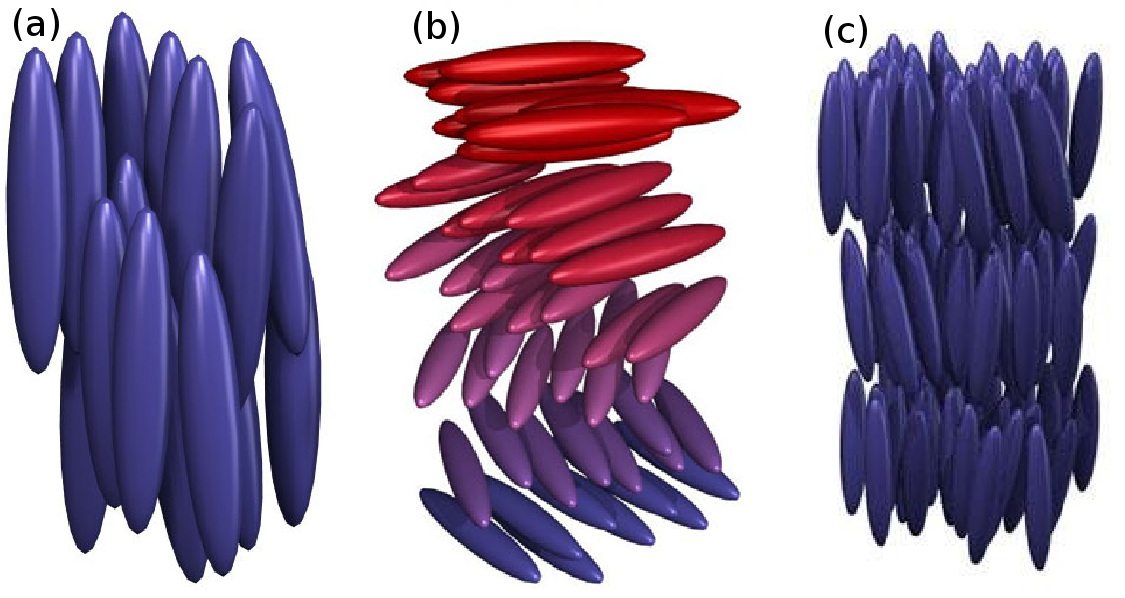
\includegraphics[width=.8\textwidth]{./Slike/faze}
 \caption{Shematski prikaz treh najpogostej"sih teko"cekristalnih mezofaz: nematik (a), kiralni nematik ali holesterik (b) in smektik (c)\cite{wiki:lc}.}
  \label{fig:faze}
\end{figure}

\subsection{Orientacijski red}

V vseh teko"cekristalnih mezofazah imajo gradniki orientacijski red dolgega dosega. Definiramo lahko enotski vektor $\mathbf{n}$, ki dolo"ca povpre"cno smer gradnikov in ga imenujemo direktor. Direktor ni pravi vektor, saj v teko"cem kristalu ne lo"cimo med smerjo $\mathbf{n}$ in $\mathbf{-n}$. Tudi "ce sami gradniki nimajo tak"sne simetrije, jo imajo njihove fluktuacije, zato lahko ureditev dobro opi"semo z direktorjem\cite{mermin}. 

\begin{figure}[h]
\begin{center}
\subfigure{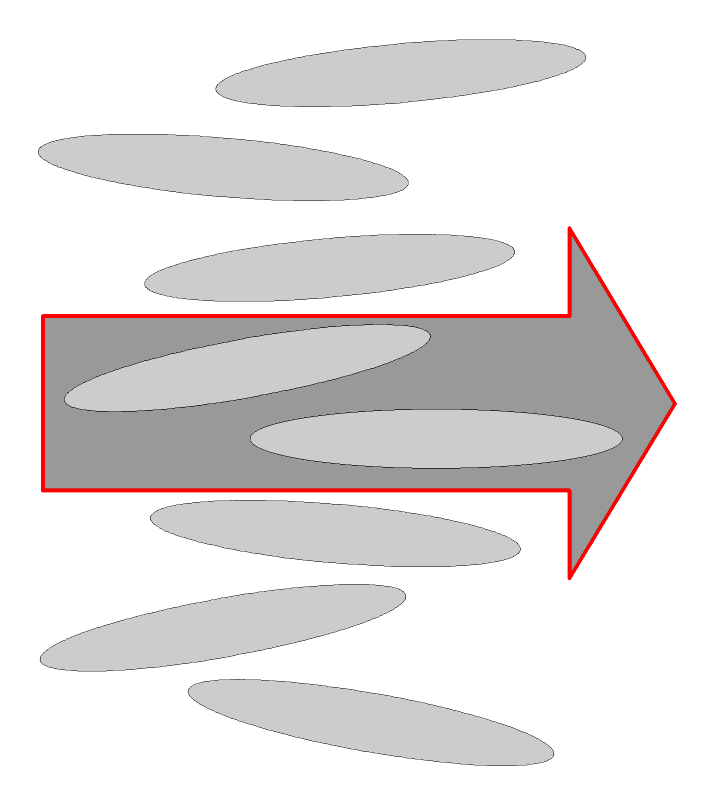
\includegraphics[height=100pt]{./Slike/Nematic-Director}}
\subfigure{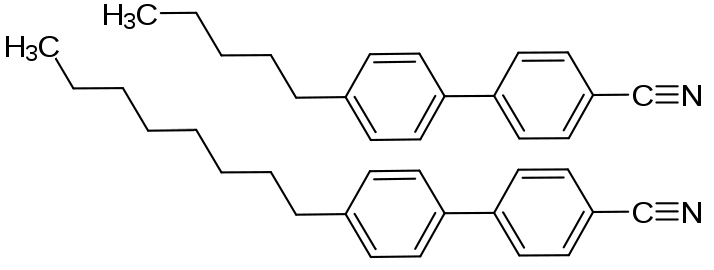
\includegraphics[height=100pt]{./Slike/nematik-formuli}}
 \caption{Levo: Gradniki imajo razli"cne orientacije, preferen"cno smer pa poda direktor. Desno: Strukturni formuli molekul 5CB (zgoraj) in 8CB (spodaj)\cite{wiki:lc}}
 \label{fig:nematik-direktor}
 \end{center}
\end{figure}

Orientacijski red dolgega dosega je tipi"cno realiziran s pali"castimi gradniki. Najpogosteje se uporabljajo organske molekule z dvema benzenovima obro"cema, na katera so vezane razli"cne skupine. Primera tak"snih molekul sta 4-ciano-4'-pentilbifenil (5CB) in 4-ciano-4'-oktilbifenil (8CB), katerih strukturni formuli sta prikazani na Sliki \ref{fig:nematik-direktor}. Velikosti tak"snih molekul so nekaj nanometrov. 

Direktor $\mathbf{n}$ podaja povpre"cno smer gradnikov, ne pa dejanske orientacije posameznih gradnikov. 
Zato uvedemo "se stopnjo reda $S$ \angl{degree of order}, ki nam pove, koliko smeri molekul v povpre"cju odstopajo od direktorja. 
Zaradi simetrije $\mathbf{n} \leftrightarrow -\mathbf{n}$ ne moremo vzeti kar povpre"cne vrednosti kota med gradnikom in direktorjem, saj je ta vrednost enaka ni"c. 
Namesto tega uporabimo povpre"cni kvadrat kota, ki je ekvivalenten kvadrupolnemu momentu\cite{kleman}
\begin{align}
 S = \frac{1}{2}\left(3\langle\cos^2\vartheta\rangle-1\right),
\end{align}
kjer je $\vartheta$ kot med osjo gradnika in direktorjem, $\langle\rangle$ pa prostorsko ali "casovno povpre"cje. 
Pri tak"sni definiciji ima popolnoma urejen teko"ci kristal, kjer so vsi gradniki vzporedni z direktorjem, vrednost $S=1$, povsem neurejen teko"ci kristal z naklju"cnimi orientacijami molekul pa $S=0$. 
V Landauovi teoriji faznih prehodov je ureditveni parameter neka koli"cina, ki je v eni fazi enaka ni"c, v drugi pa od ni"c razli"cna. 
Zgoraj definirana stopnja reda $S$ je tako primeren ureditveni parameter za prehod med izotropno teko"cino in teko"cekristalno fazo\cite{degennes}. 

Direktor in nematsko stopnjo reda lahko hkrati opi"semo z eno tenzorsko koli"cino. V ta namen uvedemo tenzor ureditvenih parametrov $Q_{ij}$ kot
\begin{align}
  Q_{ij} = \frac{S}{2}(3n_i n_j - \delta_{ij}) + \frac{P}{2}(e^{(1)}_i e^{(1)}_j - e^{(2)}_i e^{(2)}_j)\,,
\end{align}
kjer sta $\mathbf{e}^{(1)}$ in $\mathbf{e}^{(2)}$ enotska vektorja, pravokotna na $\mathbf{n}$ in med seboj. Uvedli smo "se biaksialnost $P$, ki je neni"celna, "ce fluktuacije molekul niso simetri"cne na vrtenje okrog direktorja. V tem primeru imamo orientacijski red tudi v sekundarni osi, ki je pravokotna na direktor in jo imenujemo sekundarni direktor. Parameter $P$ ima podoben pomen kot $S$ in nam pove, kako dobro so gradniki urejeni glede na sekundarno direktor. Ker komponente $n_i$ nastopajo le v kvadratu, s tak"snim zapisom avtomatsko upo"stevamo simetrijo direktorja, saj zamenjava $\mathbf{n}$ z $-\mathbf{n}$ tenzorja $Q_{ij}$ ne spremeni. Ker je $\mathbf{n}$ enotski vektor, je tenzor $Q_{ij}$ brezsleden, zato so v izotropni snovi vse njegove komponente enake 0 in je primeren ureditveni parameter za opis faznih prehodov. 

\subsection{Deformacije direktorja in prosta energija}

Ureditev teko"cega kristala lahko opi"semo s tenzorskim poljem $Q_{ij}(\vec r)$, ki podaja tenzor ureditvenih parametrov v vsaki to"cki. 
Skupno prosto energijo lahko izrazimo kot funkcional polja $Q_{ij}(\vec r)$, ki pa je odvisen od teko"cekristalne mezofaze. 
V tej nalogi obravnavamo le dve izmed mnogih teko"cekritalnih mezofaz, in sicer nematsko in holesteri"cno. 
K prosti energiji teh dveh mezofaz prispevajo elasti"cne deformacije, stopnja reda in dielektri"cna interakcija z elektri"cnim poljem. 
Drugi prispevki, npr. magnetna interakcija in fleksoelektri"cnost, so pri obi"cajno uporabljanih snoveh in opti"cnem polju zanemarljivi.

\begin{figure}[h]
\begin{center}
  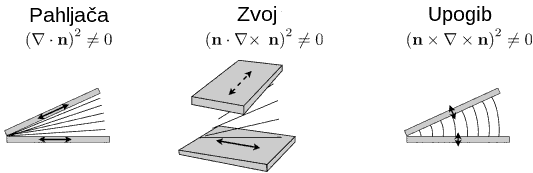
\includegraphics[width=.7\textwidth]{./Slike/tsb_slo}
  \caption{Trije na"cini elasti"cne deformacije direktorja. }
\label{fig:tsb}
\end{center}
\end{figure}
Posamezni gradniki imajo najve"cjo svobodo gibanja in s tem najve"cjo entropijo, "ce je direktor in s tem tudi teznor $Q_{ij}$ uniformen. 
Krajevno spreminjanje ureditvenega parametra $Q_{ij}$ v katerikoli smeri povzro"ci, da sistemu prosta energija naraste. 
To pove"canje je odvisno od smeri spreminjanja $Q_{ij}$ glede na smer direktorja. 
Na sliki \ref{fig:tsb} so prikazani trije na"cini deformacije direktorja, s katerimi lahko lokalno opi"semo poljubno krajevno odvisnost. 
Ti trije na"cini so pahlja"ca \angl{splay}, zvoj \angl{twist} in upogib \angl{bend}. 

V splo"snem so elasti"cne konstante, ki pripadajo vsakemu izmed treh osnovnih na"cinom deformacije, med seboj razli"cne. 
Prispevek k gostoti proste energije zaradi elasti"cnih deformacij nematskega teko"cega kristala je tako enak

\begin{align}
 f_{\mathrm{el}}^N &= \frac{K_1}{2} (\nabla \cdot \vec n)^2 + \frac{K_2}{2} (\vec n \cdot \nabla \times \vec n)^2 + \frac{K_3}{2} (\vec n \times \nabla \times \vec n)^2. 
\end{align}

\todo{tipi"cne vrednosti konstant}, \todo{izra"zava s $Q_{ij}$}

V kiralnem nematiku oz. holesteriku pa ima stanje z najni"zjo prosto energijo konstanten zvoj s periodo $a = 2\pi / q$.
Drugi "clen tako ni ve"c simetri"cen glede na smer deformacije, gostota proste energije v holesteriku pa je enaka

\begin{align}
 f_{\mathrm{el}}^{Ch} &= \frac{K_1}{2} (\nabla \cdot \vec n)^2 + \frac{K_2}{2} (\vec n \cdot \nabla \times \vec n - q)^2 + \frac{K_3}{2} (\vec n \times \nabla \times \vec n)^2. 
\end{align}

V teko"cih kristalih je stabilnost nematske mezofaze odvisna od temperature ali od koncentracije. 
Za termotropske teko"ce kristale, kjer je mezofaza odvisna od temperature, lahko zapi"semo Landauov razvoj proste energije po ureditvenem parametru $Q_{ij}$ kot
\begin{align}
  f_{\mathrm{L}} = \frac{1}{2}a(T-T^*)Q_{ij}Q_{ji} + \frac{1}{3}BQ_{ij}Q_{jk}Q_{ki} + \frac{1}{4}C(Q_{ij}Q_{ji})^2,
\end{align}
kjer je $T$ temperatura, $T^*$ najni"zja mo"zna temperatura podhlajene izotropne faze, $a$, $B$ in $C$ pa "cleni Landauovega razvoja in so odvisni od snovi. 
Ker sta konstanti $a$ in $C$ pozitivni, je pri temperaturi nad $T^*$ najugodnej"se stanje $Q_{ij}=0$ oz. $S=0$, kar ustreza izotropni snovi. 
Pri temperaturi pod $T^*$ pa kvadratni "clen zamenja predznak, zaradi "cesar postane stabilno tudi stanje z neni"celnim ureditvenim parametrom, torej nematska mezofaza. 

Na ureditev pa vpliva tudi zunanje elektri"cno polje. 
Prispevek k prosti energiji lahko razdelimo na prispevek izotropnega dela dielektri"cnega tenzorja $\overline\varepsilon$, ki ni odvisen od ureditve teko"cega kristala, in prispevka dielektri"cne anizotropije, ki predstavlja sklopitev med ureditvijo in elektri"cnim poljem. 
Skupna sprememba proste energije je enaka
\begin{align}
\label{eq:dielektricna-sklopitev}
  f_{\mathrm{EM}} = -\frac{1}{2}\varepsilon_0 \left(\overline\varepsilon E_i E_i + \frac{2}{3}\varepsilon_a^{\mathrm{mol}} Q_{ij}E_iE_j \right),
\end{align}
kjer je $\overline{\varepsilon}$ povpre"cna dielektri"cna konstanta, $\varepsilon_a^{\mathrm{mol}} = \varepsilon_{\parallel}^{\mathrm{mol}} - \varepsilon_{\perp}^{\mathrm{mol}}$ dielektri"cna anizotropija posamezne molekule, $E_i$ pa zunanje elektri"cno polje. 
"Ce na teko"ci kristal svetimo, ureditev molekul ne more slediti hitremu spreminjanju opti"cnega elektri"cnega polja, ampak nanj efektivno deluje povpre"cen kvadrat polja. 
Ta sklopitev izhaja iz polarizabilnosti molekul, ki je odvisna od njihove oblike. 
Zunanje polje v molekuli inducira elektri"cni dipolni moment, ki je sorazmeren z dol"zino molekule in je zato najve"cji, "ce je polje vzporedno z osjo molekule. 

\subsection{Defekti}

Ravnovesno stanje nematika je tak"sno, ki minimizira prosto energijo. 
V odsotnosti zunanjih polj je to ureditev z uniformnim direktorjem, kjer je celotna elasti"cna prosta energija enaka 0\cite{mermin}. 
Pod vplivom ograjenosti ali zunanjega polja pa lahko pride do stanja, kjer zvezno direktorsko polje ne more zadostiti robnim pogojem. 
V tem primeru se pojavijo obmo"cja z nedifiniranim direktorjem. 
Tak"snim obmo"cjem, kjer orientacijski red ne dr"zi, pravimo defekti. 

V treh dimenzijah lahko obstajajo to"ckasti in linijski defekti\cite{degennes,kleman}. 
V vlaknih nastopajo le linijski defekti, zato se bomo posvetili zlasti tistim. 
Linijski defekti so la"zji za razvr"s"canje, saj se lahko omejimo na ravnino, pravokotno na linijo, in problem prevedemo na dve dimenziji. 
V tem primeru lahko linijski defekt obravnavamo kot to"ckasti defekt v dveh dimenzijah. 

Disklinacije v nematskem teko"cem kristalu delimo glede na to, kako se smer direktorja spreminja v okolici disklinacije. 
Zanima nas zlasti, koliko obratov naredi direktorsko polje, "ce defekt obkro"zimo po zaklju"ceni zanki. 

\begin{figure}[h]
 \centering
 \subfigure{\includegraphics[height=100pt]{g_defect_2}}
 \subfigure{\includegraphics[height=100pt]{g_defect_-2}}
 \subfigure{\includegraphics[height=100pt]{g_defect_1}}
 \subfigure{\includegraphics[height=100pt]{g_defect_-1}}
 \caption{Nekaj mo"znih linijskih defektov. Mo"c defekta je odvisna od tega, kolikokrat se zavrti direktor (temno modre "crte), ko naredimo en krog po svetlo modrem krogu. Od leve proti desni so mo"ci 1, $-1$, $1/2$ in $-1/2$. Polcele vrednosti so mo"zne zaradi simetrije direktorja. }
\end{figure}

V dveh dimenzijah lahko nematski direktor zapi"semo kot $\vec n = (\cos\theta, \sin\theta, 0)$. 
Definiramo lahko ovojno "stevilo \angl{winding number} oz. mo"c defekta kot
\begin{align}
\label{eq:winding-number}
 s = \frac{1}{2\pi}\int_0^{2\pi} \left(\frac{d\theta}{d\phi}\right) \dd \phi
\end{align}
kjer kot $\theta$ opisuje smer direktorja, $\phi$ pa polo"zaj na na svetlo modrem krogu. 

Direktorsko polje je zvezno povsod razen v defektu, zato mora direktor pri $\phi = 0$ enak kot pri $\phi = 2\pi$. 
Ta pogoj dolo"ca mo"zne vrednosti za $s$. 
Za prava vektorska polja mora biti $s$ celo "stevilo, saj mora biti kot $\theta$ na koncu enak kot na za"cetku. 
Nematski direktor pa ima dodatno simetrijo, saj stanji $\vec n$ in $-\vec n$ predstavljata enak red. 
Zato je mo"zno, da pri obkro"zenju defekta direktor naredi le pol obrata, topolo"ski naboj $s$ pa je zato lahko tudi polcelo "stevilo. 

Vsi defekti z enakim ovojnim "stevilom so si topolo"sko ekvivalentni, saj lahko enega zvezno transformiramo v drugega. 
Zato mo"ci defekta pravimo tudi topol"ska invarianta oz. topolo"ski naboj. 
Defekti se lahko zdru"zujejo in pretvarjajo eden v drugega, skupen topolo"ski naboj pa se ohranja. 
Dva defekta z nasprotnim nabojem se lahko izni"cita, defekt z ve"cjim nabojem pa se lahko razcepi na dva defekta z manj"sim nabojem. 
Pri tem velja omejitev, da je naboj vsakega defekta lahko le polcelo "stevilo. 

Vsak defekt v teko"cem kristalu povzro"ci elasti"cno deformacijo direktorskega polja, kar pomeni zvi"sano prosto energijo sistema. 
Za linijske defekte v enokonstantnem pribli"zku je gostota elasti"cna proste energije enaka $\frac{K}{2}(\nabla \theta)^2$. 
V bli"zini defekta lahko privzamemo odvisnost $\theta(\phi) = s \phi + \theta_0$, iz "cesar sledi $\nabla\theta = \frac{k}{r}\hat e_\phi$. 
Skupni prispevek enega defekta k prosti energiji na enoto dol"zine je tako\cite{degennes}
\begin{align}
 \frac{F_d}{L} &= \frac{K}{2} \int_{r_{min}}^{r_{max}} \frac{k^2}{r^2} 2\pi r \dd r = K s^2 \pi \ln{\frac{r_{max}}{r_{min}}}
\end{align}
Zgornji izraz divergira tako v bli"zini defekta kot tudi za velike oddaljenosti. 
Velikostna skala $r_{max}$ je povezana z velikostjo sistema oz. z razdaljo do sosednjega defekta. 
En sam izoliran defekt torej nosi zelo veliko energijo, zato ni stabilen, razen "ce ga vsiljujejo robni pogoji. 
V neposredni bli"zini defekta pa je gostota proste energije tako velika, da je za teko"ci kristal bolj ugodno, da se stali v izotropno fazo. 
Velikost staljenega dela opisuje $r_{min}$. 

V zgornji enakosti je pomembna odvisnost od ovojnega "stevila. 
Elasti"cna energija zaradi defekta je sorazmerna z $s^2$, zato je bolj ugodno, da se defekt z ve"cjim ovojnim "stevilom razcepi na ve"c manj"sih defektov. 
Stabilni defekti so le tisti z ovojnim "stevilom $s=\pm1/2$, vsi ostali razpadejo na ve"c defektov z manj"sim nabojem. 

\subsection{Direktor v cilindri"cni kapilari}

Nematski teko"ci kristal se spontano uredi tako, da minimizira prosto energijo. 
V odsotnosti zunanjega polja je prosta energija najni"zja, "ce ni elasti"cnih deformacij, torej je direktor uniformen. 
V cilindri"cni geometriji s homeotropnimi robnimi pogoji pa tak"sna ureditev ni mo"zna. 
Glede na razmerja med elasti"cnimi konstantami se teko"ci kristal uredi v eno izmed konfiguracij na sliki \ref{fig:director-profiles}. 

\begin{figure}[h]
\centering
\subfigure{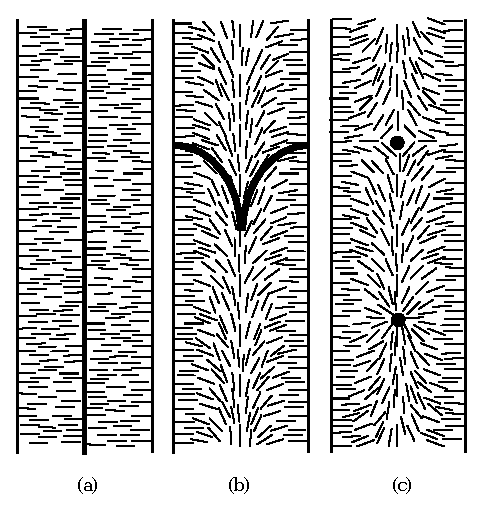
\includegraphics[height=150px]{./Slike/director-profile-cylinder-kleman}}
\subfigure{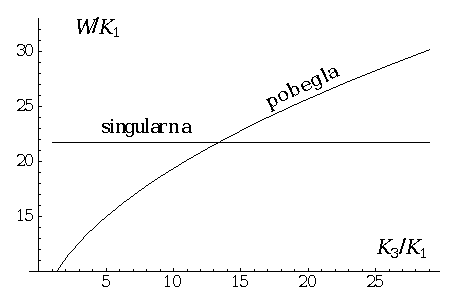
\includegraphics[clip, trim=0cm -3mm 0cm 0cm]{./Slike/escaped-director-energy}}
\caption{Levo: Prerezi valja s singularno (a) in nesingularno pobeglo disklinacijo (b). 
Razli"cne smeri pobega povzro"cijo nastanek to"ckastih singularnosti (c). Desno: Energija singularne in pobegle konfiguracije v odvisnosti od razmerja med elasti"cnima kostantama $K_1$ in $K_3$\cite{kleman}. }
 \label{fig:director-profiles}
\end{figure}

V profilu s singularno disklinacijo v osi valja je prisotna le pahlja"cna deformacija, zato je energija tega stanja odvisna od konstante $K_1$. 
V pobeglem profilu pa sta prisotni tako pahlja"cna kot upogibna deformacija. Energija tega stanja je odvisna od konstant $K_1$ in $K_3$. Do pobega pride, "ce je razmerje $K_3/K_1$ manj"se od 13, kar velja za ve"cino nematskih teko"cih kristalov. Z minimizacijo energije lahko izpeljemo ravnovesni radialni profil direktorja v cilindri"cnih koordinatah. V poenostavljenem primeru, ko sta elasti"cni konstanti $K_3$ in $K_1$ enaki, je energijsko najugodnje"se stanje\cite{kleman} 
\begin{align}
 \vec n &= (n_r, n_\phi, n_z) = (\cos \chi(r), 0, \sin \chi(r)) \\
 \chi(r) &= 2 \arctan \frac{R-r}{R+r}
\end{align}
kjer je $R$ polmer valja. Tak"sen profil je prikazan na sliki \ref{fig:director-profiles}b. V primeru pobega v tretjo dimenzijo je direktor povsod dobro definiran. "Ce pa do pobega ne pride, je tik ob osi valja defekt obmo"cje zmanj"sanega reda, kjer ureditveni parameter $S$ pade na 0. Okrog defekta je direktorsko polje radialno, torej je linijski defekt z ovojnim "stevilom $s=+1$. 

V ve"cini nematikov so vse tri elasti"cne konstante istega velikostnega reda, zato je stanje s pobegom v tretjo dimenzijo bolj ugodno. 
Veliko razmerje $K_3/K_1$ pa opazimo blizu faznega prehoda v smekti"cno fazo. 
Z uporabo 8CB, ki tvori tako nematsko kot tudi smekti"cno fazo, je mogo"ce v laboratoriju sintetizirati vlakna z radialnim profilom direktorja\cite{peddireddy}. 
Primer tvorbe tak"snih vlaken je na sliki \ref{fig:tvorjenje}. 

\begin{figure}[h]
 \centering
 \subfigure{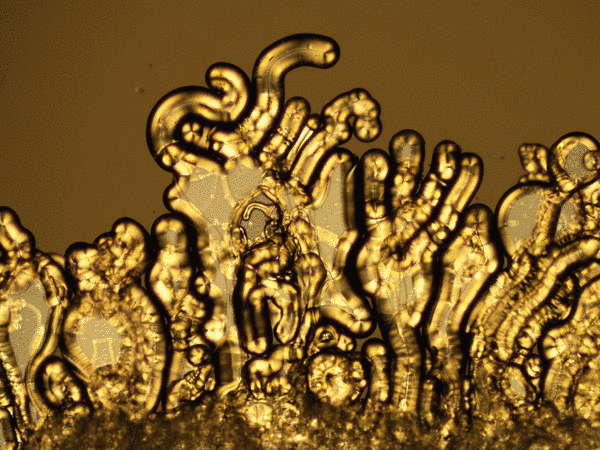
\includegraphics[height=150px]{./Slike/tvorjenje}}
 \subfigure{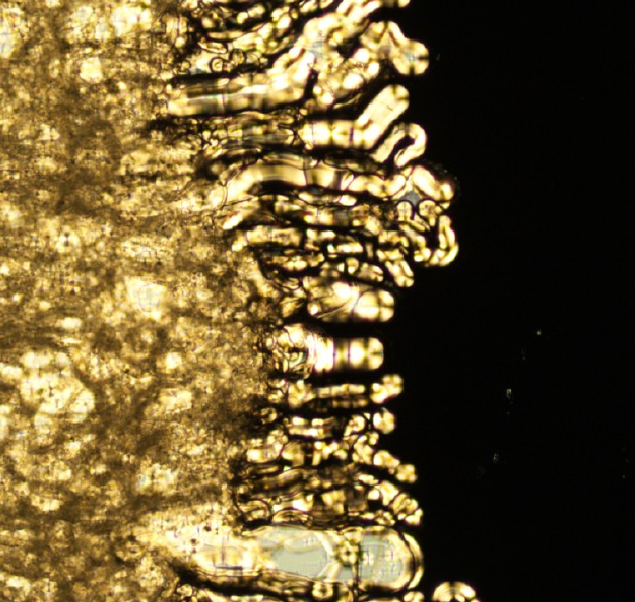
\includegraphics[height=150px]{./Slike/tvorjenje2}}
 \caption{Rast vlaken z radialnim direktorjem na meji med teko"cim kristalom 8CB in vodo\cite{peddireddy}}
 \label{fig:tvorjenje}
\end{figure}

\section{Elektromagnetno valovanje}

\subsection{Maxwellove ena"cbe v neizotropnem sredstvu}
"Sirjenje svetlobe po snovi opisujejo "stiri Maxwellove ena"cbe
\begin{equation}
\begin{aligned}
 \nabla \cdot \vec D = \rho_f & \qquad \nabla \cdot \vec B = 0 \\
 \nabla \times \vec E = -\odvod{\vec B}{t} & \qquad \nabla \times \vec H = \vec J_f + \odvod{\vec D}{t}
\end{aligned} 
\end{equation}
kjer veljata zvezi $\vec D = \varepsilon \varepsilon_0 \vec E$ in $\vec B = \mu \mu_0 \vec H$. 
V teko"cih kristalih sta dielektri"cnost $\varepsilon$ in permeabilnost $\mu$ anizotropna tenzorja. 
Obi"cajno pa je magnetna anizotropija mnogo "sibkej"sa od elektri"cne, zato jo lahko zanemarimo in privzamemo $\mu = 1$. 

Izvori in ponori valovanja znotraj vzorca so posledica neni"celne elektri"cne prevodnosti materiala.
Zaradi prevodnosti $\sigma$ ob prisotnosti elektri"cnega polja v snovi te"ce tok, ki je enak $\vec J = \sigma \vec E$. 
Prostih nabojev v vzorcu ni. Z upo"stevanjem zgornjih predpostavk lahko Maxwellove ena"cbe zapi"semo v poenostavljeni obliki
\begin{equation}
  \begin{aligned}
  \nabla \cdot \vec E = 0 & \qquad \nabla \cdot \vec B = 0 \\
  \nabla \times \vec E = -\odvod{\vec B}{t} & \qquad \nabla \times \vec B = \sigma \vec E + \varepsilon\varepsilon_0\mu_0\odvod{\vec E}{t}
  \end{aligned}
\end{equation}
V zadnji ena"cbi smo privzeli, da se dielektri"cni tenzor $\varepsilon$ ne spreminja s "casom, zato nastopa izved "casovnega odvoda. 
Ta predpostavka je smiselna pri obravnavi opti"cnih polj, saj je relaksacija teko"cega kristala mnogo po"casnej"sa od sprememb elektri"cnega in magnetnega polja. 
V tipi"cnem teko"cem kristalu in frekvencah vidne svetlobe je razlika v "casovni skali okrog 15 redov velikosti. 

\subsection{Dvolomnost}

\subsection{Defekti v polarizaciji svetlobe}
Elektri"cno in magnetno polje sta prava vektorja, zato imata lahko le defekte s celo"stevilskim ovojnim "stevilom. 
Za razliko od direktorskega polja v teko"cih kristalih pa deformacije elektromagnetih polj ne nosijo energije, zato so stabilne poljubne konfiguracije. 

Defekt v elektromagnetnem polju je to"cka oz. obmo"cje, kjer polarizacija in faza valovanja nista definirani. 
Amplituda valovanja v tak"sni to"cki mora biti enaka ni"c, zato se defekti izrazijo kot temne pege. 
Primer so Laguerre-Gaussovi snopi, prikazani na sliki \ref{fig:laguerre-gauss}. 

\begin{figure}[h]
 \centering
 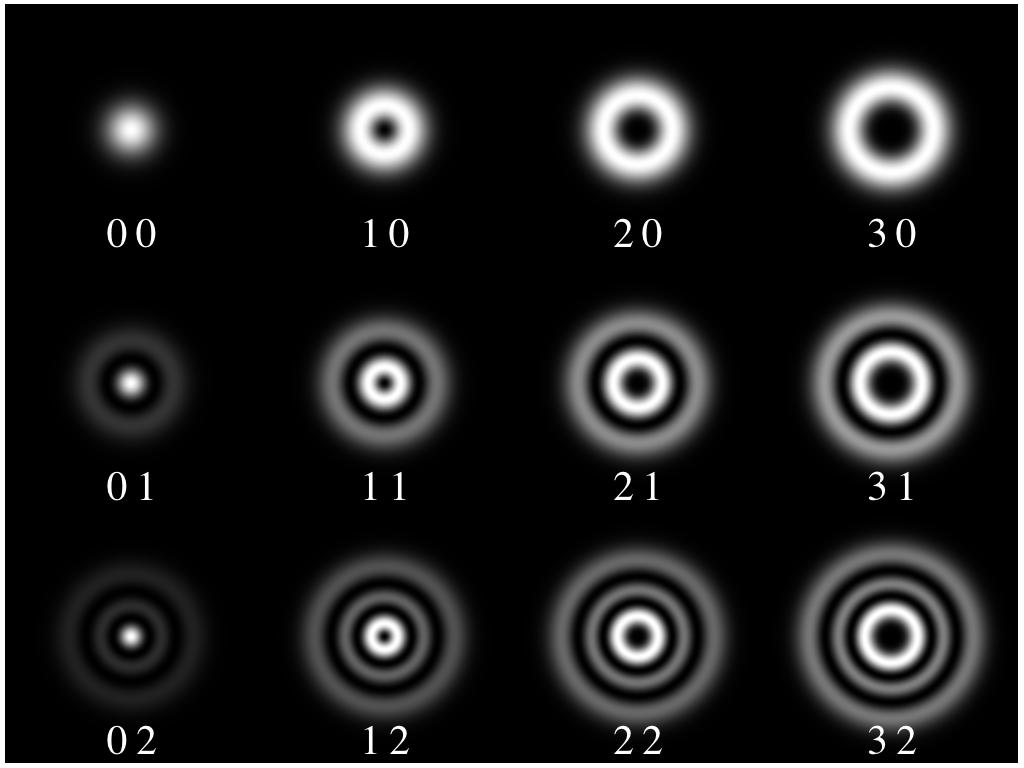
\includegraphics[width=.6\textwidth]{./Slike/LG-wiki}
 \caption{Nekaj osnovnih Laguerre-Gaussovih na"cinov. Temne pege v notranjosti snopov predstavljajo defekte v polarizaciji svetlobe. \cite{lg-wiki}}
 \label{fig:laguerre-gauss}
\end{figure}


V opti"cnih poljih je nihanje elektri"cnega in magnetnega polja tako hitro, da z nobeno merilno napravo ne moremo izmeriti samega polja, ampak le njegovo "casovno povpre"cje. 
Med polarizacijo svetlobe $\vec P$ in $-\vec P$ je razlika zgolj v fazi, zato ju lahko obravnavamo kot enaki. 
V tem smislu je polarizacija svetlobe podobna nematskemu direktorju. 
Kljub temu da z elektri"cnim poljem ne moremo skonstruirati pravega defekta s polcelim ovojnim "stevilom, imamo lahko na neki to"cki obrat polja, ki ne pove"ca proste energije. 


\section{Dielektri"cni tenzor v teko"cem kristalu}
\label{sec:dielektricnost}
Oblika in polarizabilnost molekul v teko"cem kristalu vplivata na njegove opti"cne lastnosti. 
Dielektri"cni tenzor v teko"cem kristalu je odvisen od molekularne anizotropije $\varepsilon_{a}^{\mathrm{mol}}$, direktorja in nematske stopnje reda $S$. 
Odvisnost od direktorja in stopnje reda lahko opi"semo s tenzorskim ureditvenim parametrom $Q_{ij}$. 
Ta je brezsleden, zato tudi dielektri"cni tenzor zapi"semo kot vsoto izotropnega in brezslednega tenzorja kot\cite{degennes, ravnik-zumer-ldg}

\begin{align}
\label{eq:dielektricni-tenzor}
 \varepsilon_{ij} &= \overline\varepsilon + (\varepsilon_a)_{ij} = \overline\varepsilon + \frac{2}{3}\varepsilon_a^{\mathrm{mol}} Q_{ij}
\end{align}

Lastni vektorji tenzorja $Q_{ij}$ so direktor in dve pravokotni smeri, po zgornji zvezi pa so enake tudi lastne osi dielektri"cnega tenzorja. 
V enoosnem teko"cem kristul je tako opti"cna os z izrednim lomnim koli"cnikom vzporedna z direktorjem. 

"Ce primerjamo ena"cbi (\ref{eq:dielektricna-sklopitev}) in (\ref{eq:dielektricni-tenzor}) opazimo dvosmerno povezavo med ureditvijo teko"cega kristala in elektromagnetnim poljem. 
Zaradi dielektri"cne sklopitve svetloba vpliva na ureditev teko"cega kristala, zaradi opti"cne anizotropije pa teko"ci kristal vpliva na "sirjenje svetlobe po njem. 
Ra"cunsko orodje, ki naj bi natan"cno napovedalo direktorsko polje ob prisotnosti svetlobe ali "sirjenje svetlobe skozi teko"ci kristal, bi moralo upo"stevati to dvosmerno povezavo in hkrati ra"cunati oboje. 
V praksi pa se pogosto zate"cemo k poenostavitvam oz. limitam mo"cnega ali "sibkega polja. 
"Ce je elektromagnetno polje dovolj mo"cno, se bo direktor orientiral v smeri polja, torej svetloba vedno "cuti izredni lomni koli"cnik. 
V tem re"zimu teko"ci kristal ne vpliva na "sirjenje svetlobe. 
"Ce pa je svetloba zelo "sibka, ne spremeni orientacije molekul in lahko privzamemo, da je direktorsko polje fiksirano. 
Mo"cno se razlikujeta tudi "casovni skali obeh pojavov, saj je karakteristi"cni "cas relaksacije teko"cega kristala velikostnega reda sekunde, opti"cna polja pa nihajo s periodo okrog femtosekunde. 
Zato lahko preu"cujemo propagacijo svetlobe preden se teko"ci kristal lahko preuredi. 

V tem magistrskem delu sem se omejil le na "sirjenje svetlobe, pri "cemer je direktorsko polje konstantno. 
Sama ra"cunska metoda pa je zasnovana tako, da je kompatibilna z obstoje"cimi programi za izra"cun ureditve teko"cih kristalov\cite{ravnik-zumer-ldg}. 
Z isto metodo bo v prihodnosti mogo"ce upo"stevati dvosmerno sklopitev med opti"cnim poljem in teko"cim kristalom, premostiti pa bo treba "se razliko v "casovnih skalah. 

\subsubsection{Povezava med defekti v teko"cem kristalu in defekti v opti"cnem polju}
Orientacijski red v teko"cem kristalu je tesno povezani z opti"cnimi polji. 
Med njimi obstaja dvosmerna povezava, opisana v poglavju \ref{sec:dielektricnost}. 
Podobno so med seboj povezani tudi defekti. 


\begin{comment}
 
\subsubsection{Valj z dvojnim zvojem}

Holesteri"cni teko"ci kristal ima najni"zjo prosto energijo, "ce ima stalen zvoj. 
\todo{Mogo"ce kaj vec o double-twist cylindrih}

\begin{figure}
 \centering
 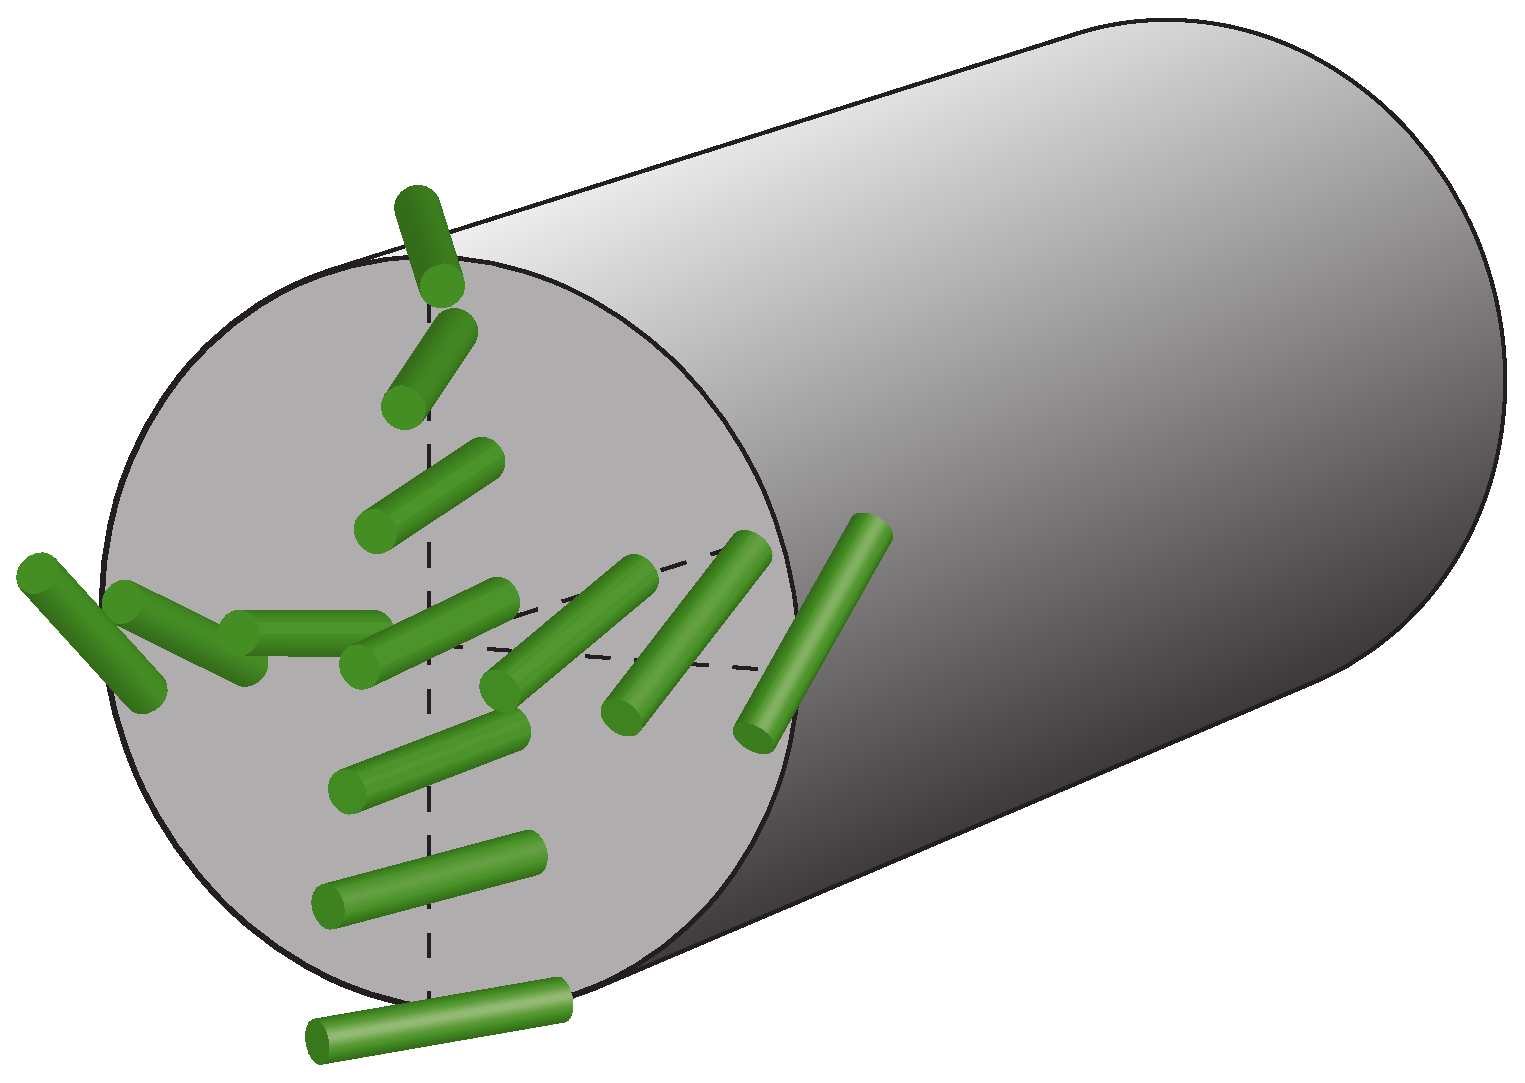
\includegraphics[width=.5\textwidth]{./Slike/double-twist-cylinder-coles-morris}
 \caption{Shematski prikaz direktorja v valju z dvojnim zvojem. Na osi valja je direktor vzporeden z osjo, z oddaljenostjo od osi pa kot med osjo in direktorjem nara"s"ca linearno\cite{coles-morris}. }
 \label{fig:double-twist-cylinder}
\end{figure}

\end{comment}

\section{Numeri"cna metoda}

Za samo ra"cunanje sem implementiral metodo kon"cnih diferenc v "casovni domeni \angl{\acf{FDTD}}\cite{taflove}. 
Pri tej metodi "casovno propagiramo elektri"cno in magnetno polje v vsaki to"cki po Maxwellovih ena"cbah. 

Pri numeri"cnem re"sevanju potrebujemo le zadnji dve ena"cbi, ki vsebujeta "casovne odvode polj. 
Prvi dve ena"cbi bosta s tem avtomatsko izpolnjeni. 
Izvore valovanja namesto z dodajanjem nabojev in tokov v vzorec raje simuliramo z robnimi pogoji, kot da valovanje prihaja od zunaj. 
Ta pristop je smiseln, saj v eksperimentih teko"ci kristal opazujemo tako, da svetimo skozenj. 

"Ce izrazimo "casovna odvoda in ena"cbi prepi"semo v brezdimenzijsko obliko ($c = \varepsilon_0 = \mu_0 = 1$), se glasita
\begin{align}
\label{eq:maxwell-base}
 \odvod{\vec{B}}{t} = -\nabla \times \vec{E}, \qquad \odvod{\vec{E}}{t} = \eps^{-1} (\nabla \times \vec{B} - \sigma \vec E)\,.
\end{align}

V zgornjih ena"cbah smo implicitno upo"stevali, da v celici ni izvorov, uporabili pa smo brezdimenzijske enote, zato je $c=1$.
V ena"cbah nastopajo le prvi odvodi, ki jih za numeri"cno ra"cunanje nadomestimo s kon"cnimi diferencami
\begin{align}
 \frac{\partial y}{\partial x} \rightarrow \frac{y(x+\delta) - y(x)}{\delta}
\end{align}

Znotraj teko"cega kristala lahko elektri"cno prevodnost zanemarimo in izpustimo "clen $\sigma \vec E$. 
Prevodnost pa je pomembna v robni plasti, kjer "zelimo absorpcijo valovanja. 

Pri ra"cunih sem upo"steval le dielektri"cno anizotropijo teko"cega kristala, magnetno pa zanemaril. 
Zaradi simetrije Maxwellovih ena"cb bi na enak na"cin kot dielektri"cnost $\varepsilon$ lahko upo"steval tudi magnetno permeabilnost $\mu$. 
Podobno bi lahko poleg elektri"cne prevodnosti $\sigma$ upo"steval magnetne izgube $\sigma^*$. 

\subsection{Mre"za}

Pri diskretizaciji si lahko pomagamo z obliko obeh ena"cb. 
Za izra"cun "casovnega odvoda vsakega izmed polj $\vec{E}, \vec{B}$ potrebujemo le vrednosti drugega polja. 
Poleg tega obe ena"cbi povezujeta "casovni odvod enega polja s krajevnim odvodom drugega. 
Zaradi obeh opisanih lastnosti lahko dvignemo red metode, in s tem izbolj"samo natan"cnost, "ce vrednosti polj poznamo ob razli"cnih "casih in na razli"cnih mestih\cite{taflove}. 

Obi"cajne implementacije metode \acs{FDTD} gredo "se korak dlje, tako da so tudi posamezne komponente elektri"cnega in magnetnega polja definirane na razli"cih to"ckah\cite{yee, yee-lattice}.
Tak"sno mre"zo je predlagal Yee in izkori"s"ca dejstvo, da pri "casovnem odvodu vsake komponente posameznega polja nastopata le krajevna odvoda ostalih dveh komponent drugega polja. 
Z ustrezno izbiro to"ck, kjer so definirane posamezne komponente, so vsi krajevni odvodi izra"cunani ravno na sredini med ustreznima to"ckama mre"ze. 
Za u"cinkovito delovanje pa tak"sna mre"za zahteva, da je dielektri"cni tenzor $\eps$ diagonalen, njegove komponente pa morajo biti znane na razli"cnih to"ckah mre"ze. 
V praznem prostoru ali v trdnih kristalih temu pogoju lahko zadostimo, po mo"znosti z vrtenjem koordinatnega sistema.

V teko"cih kristalih je dielektri"cni tenzor anizotropen in se mo"cno spreminja s krajem. 
Zaradi krajevnega spreminjanja ne moremo tako obrniti koordinatnega sistema, da bi bil tenzor diagonalen v vseh to"ckah. 
Poleg tega obstoje"ci programi za modeliranje ureditve teko"cih kristalov podajo vse komponente dielektri"cnega tenzorja na istem mestu\cite{ravnik-zumer-ldg}.
Odlo"cil sem se za srednjo pot, kjer sta polji $\E$ in $\B$ definirani ob razli"cnih "casih in na razli"cnih to"ckah mre"ze, vse tri komponente vsakega izmed polj pa so podane na istem mestu. 
Obe mre"zi prikazuje slika \ref{fig:lattice}. 

\begin{figure}[h]
\centering
 \subfigure{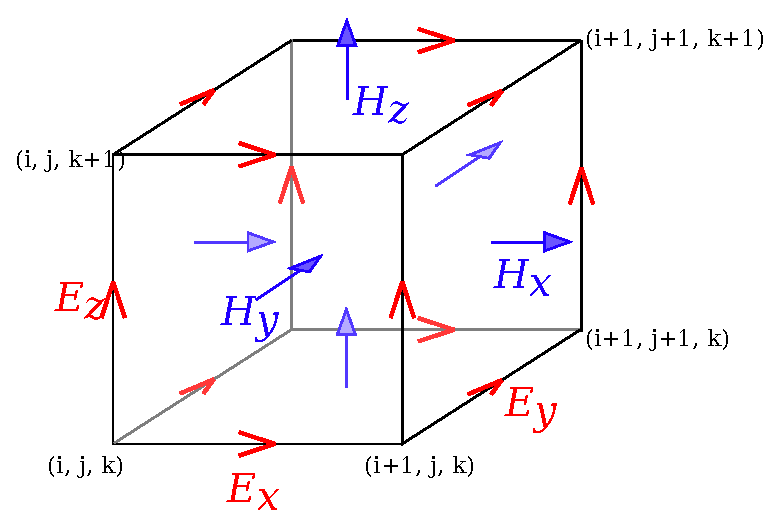
\includegraphics[width=.5\textwidth]{./Slike/Yee-cube}}
 \subfigure{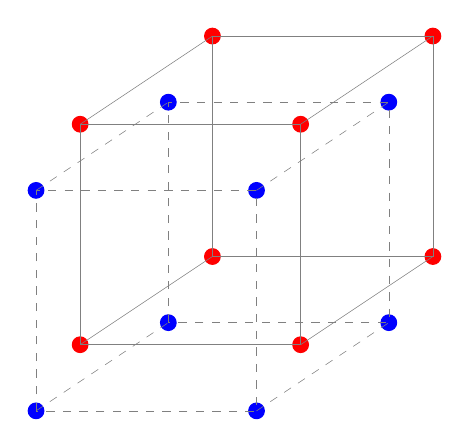
\begin{tikzpicture}[scale=1.4]
    
    \foreach \x in {0,1}{
      \foreach \y in {0,1}{
        \node[mpoint] at (2*\x,2*\y) {}; 
        \node[mpoint] at (2*\x+1.2,2*\y+0.8) {}; 
        \node[epoint] at (2*\x+1.6,2*\y+1.4) {};
        \node[epoint] at (2*\x+1.6-1.2,2*\y+1.4-0.8) {};
        \draw[mgrid] (2*\x,2*\y) -- (2*\x+1.2,2*\y+0.8);
        \draw[egrid] (2*\x+1.6,2*\y+1.4) -- (2*\x+1.6-1.2,2*\y+1.4-0.8);
      }
    }
    
    \draw[mgrid] (0,0) rectangle (2,2);
    \draw[mgrid] (1.2,0.8) rectangle (3.2,2.8);
    \draw[egrid] (1.6,1.4) rectangle (3.6,3.4);
    \draw[egrid] (1.6-1.2,1.4-0.8) rectangle (3.6-1.2,3.4-0.8);

            \end{tikzpicture}}
\caption{Levo: Yeejeva celica, pri kateri so komponente elektri"cnega polja znane na razpolovi"s"cih robov konce, komponente magnetnega polja pa v sredi"s"cih ploskev\cite{yee-lattice}. Desno: Celica, ki sem jo uporabil pri izra"cunih. Komponente elektri"cnega polja so znane v ogli"s"cih kocke, komponente magnetnega polja pa v njenem sredi"s"cu. V obeh primerih sta elektri"cno in magnetno polje dolo"cena ob razli"cnih "casih, kar na sliki ni prikazano.}
\label{fig:lattice}
\end{figure}

Za ra"cun potrebujemo "se inverz dielektri"cnega tenzorja, ki pa se med propagacijo svetlobe ne spreminja, zato ga lahko izra"cunamo predhodno. 
Pomembno je le, da je znan na istem mestu kot $\E$ (rde"ce to"cke na sliki \ref{fig:lattice}), vendar ob "casu, ko je podan $\B$. 

\subsection{Ena"cbe}

Na izbrani mre"zi ne moremo neposredno izra"cunati rotorja polj, ker ta ni definiran v pravih to"ckah. 
Elektri"cno polje je definirano na ogli"s"cih kocke, zato so krajevni odvodi tega polja definirani na razpolovi"s"cih robov, potrebujemo pa jih na mestu magnetnega polja, torej v sredi"s"cu kocke. 
V svoji metodi sem za odvod polja po vsaki koordinati v sredi"s"cu kocke uporabil povpre"cje odvodov na vseh "stirih robovih, ki potekajo v smeri izbrane koordinate, kot prikazuje slika \ref{fig:lattice-derivatives}. 

\begin{figure}[h]
\centering
 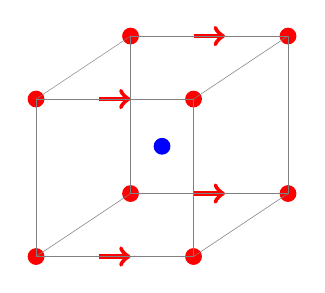
\begin{tikzpicture}
  \foreach \y in {0,1}{
      \foreach \x in {0,1}{
        \node[epoint] at (2*\x+1.6,2*\y+1.4) {};
        \node[epoint] at (2*\x+1.6-1.2,2*\y+1.4-0.8) {};
        \draw[egrid] (2*\x+1.6,2*\y+1.4) -- (2*\x+1.6-1.2,2*\y+1.4-0.8);
      }
      \draw[->,red,ultra thick] (1.4+1,2*\y+1.4) -- +(0.4,0);
      \draw[->,red,ultra thick] (0.2+1,2*\y+0.6) -- +(0.4,0);
    }
    
    \draw[egrid] (1.6,1.4) rectangle (3.6,3.4);
    \draw[egrid] (1.6-1.2,1.4-0.8) rectangle (3.6-1.2,3.4-0.8);
    
    \node[mpoint] at (2,2) {};
 \end{tikzpicture}
 \caption{
 Krajevni odvodi komponent polja $\E$ v smeri $x$ so definirani na "stirih robovih, ozna"cenih s pu"s"cicami. 
 Vrednost potrebujemo v sredi"s"cu kocke (modra pika), zato sem uporabil povpre"cje "stirih vrednosti na robu. 
 }
 \label{fig:lattice-derivatives}
\end{figure}

V primerjavi z Yeejevo celico povpre"cenje pove"ca "cas ra"cunanja, saj moramo namesto vsakega krajevnega odvoda izra"cunati "stiri. 
Na sre"co pa si vsah rob delijo "stiri kocke, tako da se s sprotnim shranjevanjem odvodov lahko izognemo ve"ckratnemu ra"cunanju istega odvoda. 
Na ta na"cin je "stevilo ra"cunskih operacij blizu tistemu, ki bi ga potrebovali z uporabo Yeejeve mre"ze. 

\subsection{Izvor valovanja}

V ena"cbah (\ref{eq:maxwell-base}) ne nastopajo izvori valovanja, zato jih moramo moramo modelirati z robnimi pogoji. 
To je v skladu z eksperimenti, saj svetloba pride od zunaj, zanima pa nas predvsem njeno "sirjenje skozi snov. 

Poljubno vpadno valovanje lahko modeliramo z robnimi pogoji, "ce izkoristimo linearnost Maxwellovih ena"cb. 
Elektri"cno in magnetno polje lahko namre"c razcepimo na vsoto vpadnega in sipanega valovanja\cite{taflove}. 
Tak"sen razcep polja je mo"zen le, "ce je "sirjenje vpadnega valovanja dobro znano. 
Mre"zo zato razdelimo na dve obmo"cji, v notranjem obmo"cju ra"cunamo s skupnim poljem, v zunanjem pa polje razcepimo in shranjujemo le sipani del.
Opti"cno anizotropna snov mora biti v celoti v notranjem obmo"cju, izvor valovanja modeliramo na prehodu med obmo"cjema. 

\begin{figure}[h]
 \centering
 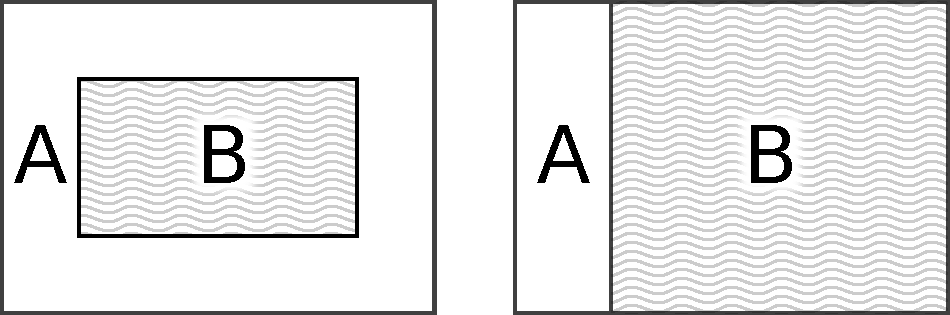
\includegraphics[width=.8\textwidth]{./Slike/wave-source-regions}
 \caption{Delitev mre"ze na dve obmo"cji. V obmo"cju \textbf{A} ra"cunamo le z sipanim valovanjem, v obmo"cju \textbf{B} pa s celotnim valovanjem. Delitev na levi sliki je primerna, "ce je razlika med lomnima koli"cnikoma \textbf{A} in \textbf{B} dovolj majhna. V nasprotnem primeru uporabimo delitev na desni sliki. }
 \label{fig:wave-source-regions}
\end{figure}

Delitev na notranje in zunanje obmo"cje je u"cinkovita, "ce se efektivni lomni koli"cnik v notranem obmo"cju ne razlikuje mo"cno od zunanjega. 
V tem primeru je fazna razlika na zadnji stranici notrenjega obmo"cja dovolj majhna, da pretvorba na sipano valovanje odstrani ve"cino valovanja. 
"Ce pa je fazna razlika primerljiva s $\pi/2$ ali ve"cja, lahko odstranitev vpadnega vala celo pove"ca amplitudo valovanja. 
To se zgodi npr. v teko"cekristalnem valovodu, ki je mnogo dalj"si od valovne dol"zine svetlobe. 
Takrat je bolj u"cinkovito upo"stevati izvor valovanja le na vpadni strani. 

Delitev na zunanje in notranje obmo"cji, ki je prikazana na levi strani slike \ref{fig:wave-source-regions}, sem uporabil le s preprostimi primeri za preverjanje delovanja metode. 
Vse ostale izra"cune sem izvajal z delitvijo na desni strani. 
Na sliki je velikost obmo"cja \textbf{A} pretirana zaradi preglednosti. 
V vseh primerih je bila debelina obmo"cja \textbf{A} enaka dva koraka mre"ze. 

\subsection{Robni pogoji}

"Ce imamo na robu celice Dirichletov, Neumannov ali me"sani robni pogoj, se bo celotno valovanje odbilo in vrnilo v celico. 
Tega si ne "zelimo, pri izvedbi ekperimentov obi"cajno svetloba najprej preide skozi vzorec, nato pa jo zajamemo in preu"cimo. 
To lahko simuliramo z uporabo absorbirajo"cega robnega pogoja \angl{\ac{ABC}}. 
Obstaja ve"c razli"cnih implementacij absorbirajo"cih robnih pogojev, v zadnjem "casu se najve"c uporablja t.i. popolnoma ujemajo"ca plast \angl{\ac{PML}}\cite{taflove,berenger}. 

Material v plasti \acs{PML} zagotavlja eksponentno pojemanje vpadnega vala, neodvisno od njegove frekvence in smeri "sirjenja. 
Absorpcijo valovanja dose"zemo z uporabo elektri"cne prevodnosti $\sigma$ in magnetnih izgub $\sigma^*$. 
Odboju na meji med notranjostjo celice in plastjo \acs{PML} se izognemo, "ce izgube v robni plasti zado"s"cajo pogoju $\sigma/\sigma^* = \eps_1/\mu_1$, kjer sta $\eps_1$ in $\mu_1$ dielektri"cnost in magnetna permeabilnost v notranjosti. 
To ujemanje izgub odpravi odboj na meji le za valovanje, ki vpada pravokotno na mejo. 
Odboj valovanja pod poljubnim kotom prepre"cimo, "ce vsako komponento elektri"cnega in magnetnega polja razdelimo na dva prispevka. 
Tak material je nefizikalen, saj imamo dodatne prostostne stopnje, polje pa ne sledi ve"c Maxwellovim ena"cbam. 

Komponenta $E_x$ elektri"cnega polja vala v obi"cajnem mediju z dielektri"cnostjo $\eps$ in elektri"cno prevodnostjo $\sigma$ zado"s"ca Maxwellovi ena"cbi

\begin{align}
 \eps \odvod{E_x}{t} + \sigma E_x = \odvod{H_z}{y} - \odvod{H_y}{z}\;.
\end{align}

V plasti \acs{PML} pa elektri"cno polje razdelimo na dva prispeka, $E_x = E_{xy} + E_{xz}$, ki zado"s"cata ena"cbam

\begin{align}
 \eps \odvod{E_{xy}}{t} + \sigma_y E_{xy} &= \odvod{}{y}(H_{zx} + H_{zy}) \\
 \eps \odvod{E_{xz}}{t} + \sigma_z E_{xz} &= -\odvod{}{z}(H_{yx} + H_{yz})\;,
\end{align}

kjer smo razcepljenima komponentoma pripisali razli"cni prevodnosti. 
Na enak na"cin so razcepljene ostale komponente eletri"cnega in magnetnega polja. 

\subsection{Opis valovoda}



\section{Preverjanje metode}

\todo{Test z dejasnkim profilom, ki ga imajo v opti"cnih vodniki}

\subsection{Prazen prostor}
Prvi preizkus metode, ki sem ga opravil, je "sirjenje svetlobe skozi prazen prostor. 
Prazen prostor sem modeliral kot snov, kjer je dielektri"cni tenzor uniformen in izotropen. 
"Ce na eno stran celice postavimo planarni izvir ravnega valovanja, pri"cakujemo ravne valove po celotnem mediju. 

Pri tem preizkusu sta lomna koli"cnika v obeh obmo"cjih enaka, zato sem mre"zo razdelil na notranje in zunanje obmo"cje, izvor valovanja pa sem postavil po celotnem robu med obmo"cjema. 
Prikaz valovanja na sliki \ref{fig:test-plane} potrjuje pravilnost metode, saj res vidimo ravne valove s konstantno frekvenco in valovno dol"zino. 

\begin{figure}[h]
 \centering
 \subfigure{\includegraphics[width=.45\textwidth]{g_test_plane}} \,
 \subfigure{\includegraphics[width=.45\textwidth]{g_test_plane_profile}}
\caption{Levo: Trenutna slika valovanja v celici. Desno: "Casovna in krajevna odvisnost valovanja. \todo{Bolj"si opis, pu"s"cice na slikah}}
\label{fig:test-plane}
\end{figure}

Na obeh slikah opazimo notranjost celice z valovanje in rob, kjer valovanja ni.
To je posledica modeliranja izvora valovanja okrog in okrog celice, kot je prikazano na levi strani slike \ref{fig:wave-source-regions}.
Valovanje se "siri od leve proti desni, tako si lahko predstavljamo izvir valovanja ne levi strani in ponor na desni. 
Dejstvo, da ponor valovanja na desni strani uspe"sno pobere celotno valovanje potrjuje natan"cnost ra"cunanja. 

\subsection{Lom in odboj}
Enostaven preizkus za "sirjenje valovanja je prehod "cez mejo med medijema z razli"cnima lomnima koli"cnikoma. 
Del valovanja se na meji odbije po odbojnem zakonu, tako da je odbojni kot enak vpadnemu. 
Preostanek valovanja se na meji lomi, lomni kot pa je odvisen od lomnih koli"cnikov obeh snovi. 
Izra"cunamo ga po lomnem zakonu
\begin{align}
 \frac{\sin\alpha}{\sin\beta} &= \frac{n_2}{n_1} = \sqrt{\frac{\varepsilon_2}{\varepsilon_1}}\;, 
\end{align}
kjer je $\alpha$ vpadni kot valovanja, $\beta$ pa lomni kot oz. kot med pravokotnico in smerjo "sirjenja lomljenega vala. 

Dele"za odbitega in prepu"s"cenega valovanja sta odvisna od vpadnega kota $\alpha$ in polarizacije svetlobe\cite{wiki:brewster}. 
Pri dolo"cenem kotu $\alpha$ se komponenta svetlobe s polarizacijo v ravnini "zarka in normale na povr"sino ne odbije in se v celoti lomi. 
Tamu kotu re"cemo Brewsterjev kot in je enak
\begin{align}
 \theta_B &= \arctan\left(\frac{n_2}{n_1}\right) = \arctan\sqrt{\frac{n_2}{n_1}}
\end{align}

"Ce propagacijo svetlobe simuliramo z metoda \ac{FDTD}, v sliki trenutnega elektri"cnega polja ne moremo lo"citi med vpadnim in odbitim valovanjem. 
Za prikaz delovanja sem zato uporabil vpadni kot, ki je zelo blizu Brewsterjevemu. 
Na ta na"cin opazimo le "sibko odbito valovanje, tako da lahko "se vedno preverimo, ali lomni zakon dr"zi. 
Slika elektri"cnega polja ob prehodu meje v bli"zini Brewsterjevega kota je na sliki \ref{fig:refraction-test}. 

\begin{figure}[h]
 \centering
 \input{g_refraction_test}
 \vspace{-1.7cm}
 \caption{Preizkus veljavnosti lomnega zakona ob prehodu valovanja v medij z druga"cnim lomnim koli"cnikom}
 \label{fig:refraction-test}
\end{figure}

Na sliki so jasno vidna "stiri obmo"cja. "Cisto na levi je rob z absorbirajo"cim robnim pogojem \ac{PML}, ki absorbira odbito valovanje in prepre"cuje nadaljnji odboj. 
Naslednje je obmo"cje z dielektri"cnostjo $\varepsilon_1$, kjer je superpozicija vpadnega in odbitega valovanja. 
Odbito valovanje je mnogo "sibkej"se od vpadnega, zato so valovi skoraj ravni. 
Na sredini slike je meja med obmo"cjema, desno od nje je snov z dielektri"cnostjo $\varepsilon_2 > \varepsilon_1$.
V tem delu je le prepu"s"ceno lomljeno valovanje, ki ima ustrezno manj"so valovno dol"zino. 
Na desnem robu je prazno obmo"cje, ki ga valovanje "se ni doseglo. 

Veljavnost lomnega zakona lahko preverimo, "ce primerjamo kota vpadnega in lomljenega valovanja. 
Dol"zini stranic na sliki nista v enakem merilu, zato kotov ne moremo od"citati s slike. 

\todo{Simuliraj lom na novo, izracunaj oba kota}


\subsection{Uniformen direktor}
Za naslednji preizkus sem simuliral dvolomni kristal, torej snov, kjer je dielektri"cni tenzor uniformen, ne pa tudi izotropen. 
Svetloba se je "sirila v smeri osi $z$, opti"cna os pa je oklepala kot $\theta$ z ravnino $x$-$y$ in kot $\beta$ s polarizacijo vpadne svetlobe. 
Preu"ceval sem prepustnost tak"snega sistema, "ce za celico postavimo polarizator, ki je pravokoten na polarizacijo vpadne svetlobe. 

Ta preizkus temelji na najpogosteje uporabljani metodi za eksperimentalno opazivanje teko"cih kristalov. 
Tanko plast teko"cega kristala postavimo med dva prekri"zana polarizatorja. 
"Ce je med polarizatorjema opti"cno izotropna snov, ali pa je opti"cna os vzporedna z enim izmed polarizatorjev, sistem ne prepu"s"ca svetlobe. 
V ostalih primerih pa vidimo nekaj prepu"s"cene svetlobe, njena intenziteta je odvisna od dvolomnosti in orientacije vmesne snovi. 
Na ta na"cin se jasno vidijo defekti v teko"cem kristalu. 

"Ce je direktor uniformen po celotni debelini vzorca, lahko intenziteto prepu"s"cene svetlobe izpeljemo analiti"cno\cite{kleman}. Enaka je
\begin{align}
 I &= I_0 \sin^2 2\beta \sin^2 \left[ \frac{\pi d}{\lambda_0} \left( \frac{n_o n_e}{\sqrt{n_e^2 \cos^2 \theta + n_0^2 \sin^2 \theta}} - n_o \right)\right],
\end{align}
kjer sta $I_0$ in $\lambda_0$ intenziteta in valovna dol"zina vpadne svetlobe, $d$ debelina vzorca, $n_o$ in $n_e$ pa redni in izredni lomni koli"cnik. 
Ujemanje rezultatov z napovedjo je prikazano na sliki \ref{fig:test-uniform}.
\todo{vnesi parametre v graf}

\begin{figure}[h]
 \input{g_test_uniform}
 \caption{Rezultati preizkusa z uniformnim in anizotropnim dielektri"cnim tenzorjem}
 \label{fig:test-uniform}
\end{figure}

Na sliki vidimo zelo dobro ujemanje med simulacijo in teoreti"cno napovedjo. 
To potrjuje pravilno delovanje metode v opti"cno anizotropni snovi. 

\subsection{Periodi"cna modulacija}

%bandgap => prepovedani pas, energijska re"za
Pri periodi"cni modulaciji lomnega koli"cnika opazimo pojav, da se svetloba dolo"cenih frekvenc ne more "siriti po mediju\cite{joannopoulos}. 
Temu pojavu pravimo prepovedani pas \angl{band gap} in je soroden elektronski energijski re"zi pri molekulskih kristalih. 
Za prisotnost fotonskega prepovedanega pasu pa potrebujemo kristal oz. periodi"cno strukturo, kjer je perioda primerljiva z valovno dol"zino svetlobe. 
Fotonsko energijsko re"zo za vidno svetlobo zato opazimo pri koloidnih kristali, ki imajo periodo okrog 1 $\mu$m. 


"Sirina in oblika prepovedanega pasu sta odvisni od obeh lomnih koli"cnikov, periode modulacije in velikosti kristala. 
Za preverjanje metode sem modeliral kristal, kjer se izmenjujejo plasti z izotropno dielektri"cnostjo $\varepsilon_1$ in $\varepsilon_2$. 
Tak"sna struktura je prikazana na sliki \ref{fig:periodic-structure}. 

\begin{figure}[h]
 \centering
 \input{./Slike/periodic-structure.pdf_tex}
 \caption{Periodi"cna struktura, kjer se izmenjujeta plasti z razli"cnima dielektri"cnima konstantama. 
 Svetloba se "siri v smeri osi $z$\cite{joannopoulos}. }
 \label{fig:periodic-structure}
\end{figure}

Teoreti"cen izra"cun odvisnosti frekvence $\omega$ od valovnega vektorj $k$ je prikazan na sliki \ref{fig:joannopoulos-crystal}. 
"Ce se dielektri"cni konstanti obeh plasti razlikujeta, opazimo interval frekvenc, pri katerih ni mo"zen noben valovni vektor, torej se valovanje ne more "siriti skozi kristal. 
S pove"cevanjem razlike v dielektri"cnosti plasti se prepovedani pas raz"siri. 

\begin{figure}[h]
\centering
  \input{./Slike/bandgap.pdf_tex}
 \caption{Pojav energijske re"ze v fotonskem kristalu. Levo: celotna plast ima dielektri"cnost $\varepsilon = 13$. Sredina: Izmenjevanje plasti z dielektri"cnima konstantama 13 in 12. Desno: Izmenjevanje plasti z dielektri"cnima konstantama 13 in 1. \cite{joannopoulos}}
 \label{fig:joannopoulos-crystal}
\end{figure}

Po napovedi naj bi bila spodnja meja prepovedani pasu okrog $\frac{\omega a}{2\pi c} \approx 0,\!15$, kjer je $a$ perioda kristala, $c$ pa hitrost svetlobe. 
Zgornja meja je mo"cneje odvisna od razlike v dielektri"cnosti\cite{joannopoulos}. 

Za modeliranje tak"snega kristala sem uporabil periodi"cne robne pogoje v smereh $x$ in $y$, v smeri $z$ pa celico dol"zine 1024 enot z 20 enotami absorbirajo"ce plasti na vsakem koncu. 
Grafa prepustnosti kristalov z razli"cnimi izbirami za dielektri"cnosti sta na sliki \ref{fig:test-periodic}. 

\begin{figure}[!h]
 \input{g_test_periodic}
 \caption{Rezultati preizkusa s periodi"cno modulacijo lomnega koli"cnika}
 \label{fig:test-periodic}
\end{figure}

Na sliki res opazimo oster padec prepustnosti v dolo"cenem frekven"cnem pasu, ki se dobro ujema s pri"cakovanim na sliki \ref{fig:joannopoulos-crystal}. 
Metoda torej pravilno napove polo"zaj in "sirino prepovedanih pasov. 
Zlasti pri veliki razliki v dielektri"cnosti plasti meja prepovedanega pasu ni ostra, ampak krivulja postane zaobljena. 
To je posledica kon"cne velikosti sistema, saj so teoreti"cni izra"cuni napravljeni za neskon"cen kristal, z metodo \acs{FDTD} pa lahko modeliramo le kon"cnega. 
Kljub temu pa metoda da kvalitativno in kvantitativno pravilne rezultate za pojav fotonskega prepovedanega pasu. 

\subsection{Dvolomno vlakno}
V magistrskem delu sem preu"ceval "sirjenje svetlobe po cilindri"cnih vlaknih z razli"cnimi profili direktorja. 
Ra"cunsko metodo sem preizkusil na sistemu, ki je "cimbolj podoben obravnavanim, "se vedno pa lahko napovemo rezultat. 
V ta namen sem modeliral cilindri"cno vlakno, v katerem je uniformen dvolomen kristal, vanj pa sem posvetim s kratkim laserskim sunkom. 
Polarizacija vpadne svetlobe je bila nagnjena za 45\degree~glede na opti"cno os, tako da se je vpadni "zarek razcepil na redno in izredno komponento. 
Zaradi dvolomnosti obe komponenti potujeta z razli"cnima hitrostma, tako da se laserski "zarek razdeli na dva dela. 
Direktorsko polje je regularno, brez defektov, zato ne pri"cakujemo defektov v polarizaciji svetlobe. 

Simuliral sem zelo kratek laserski pulz, ki je trajal le nekaj valovnih dol"zin svetlobe. 
Na ta na"cin sta se obe komponenti znotraj vlakna jasno lo"cili in sem ju lahko primerjal. 
Ker se sunek hitro razcepi je tak"sen postopek primeren za iskanje lastnih na"cinov "sirjenja po valovodih\cite{taflove}. 

\begin{figure}[h]
 \centering
 \subfigure{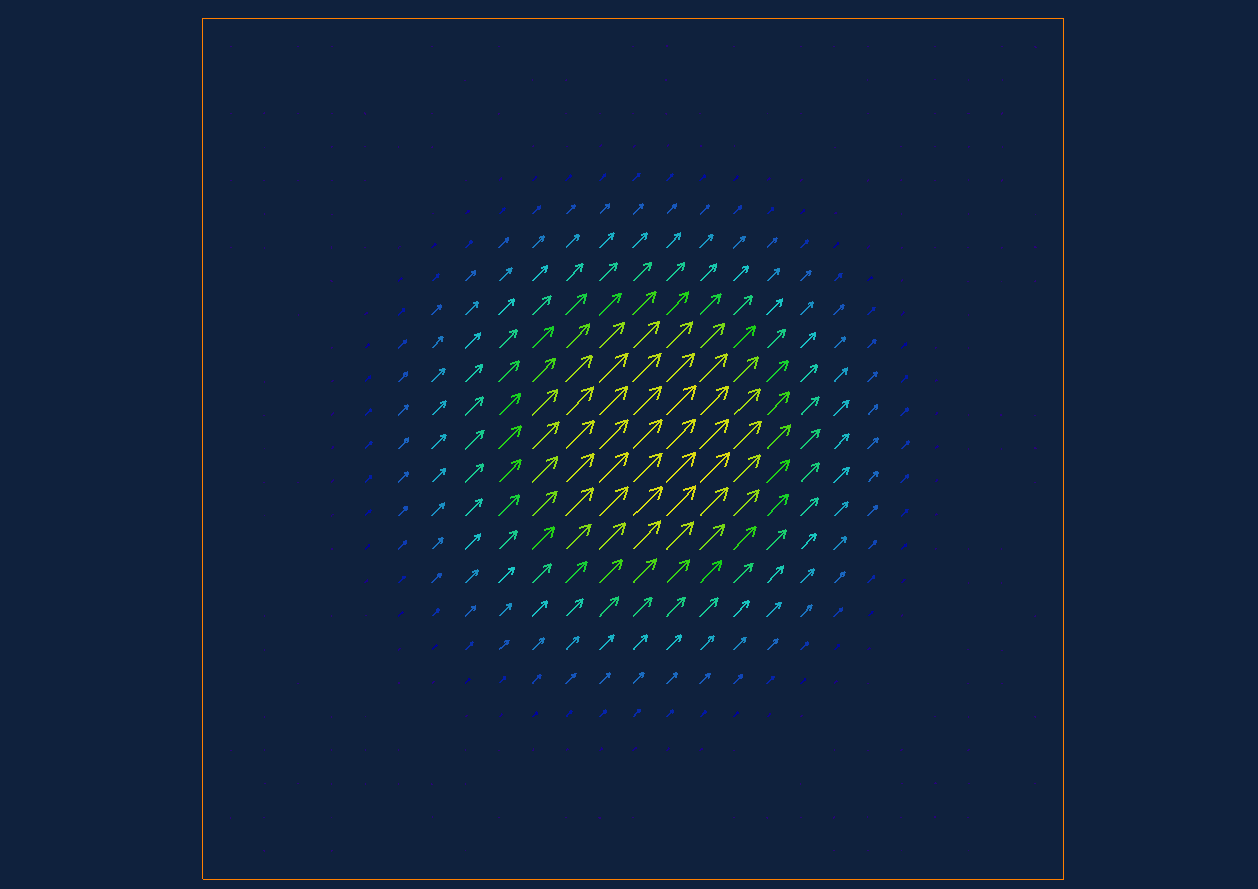
\includegraphics[width=.48\textwidth,clip,trim=5.5cm 1cm 5.5cm 1cm]{./Rezultati/0_mode1}}
 \subfigure{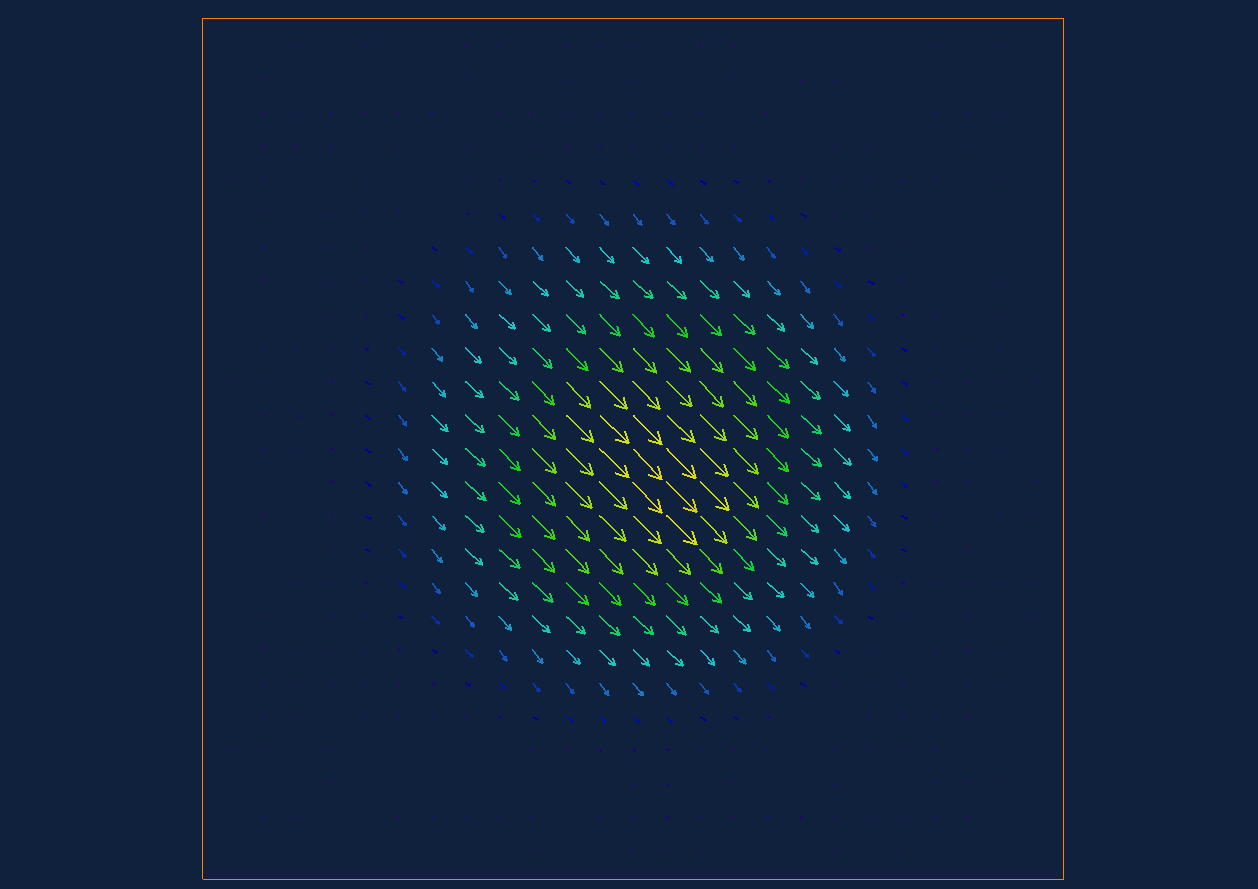
\includegraphics[width=.48\textwidth,clip,trim=5.5cm 1cm 5.5cm 1cm]{./Rezultati/0_mode2}}
 \caption{Lastna na"cina "sirjenja svetlobe skozi vlakno z uniformnim profilom direktorja. Vpadna svetloba je polarizirana vodoravno, opti"cna os pa z vodoravnico oklepa kot 45\degree. }
 \label{fig:pulse-0-mode}
\end{figure}

Rezultati na sliki \ref{fig:pulse-0-mode} potrjujejo pravilno delovanje metode. 
Vpadnja svetloba se razcepi na komponenti z redno in izredno polarizacijo, ki se "sirita z razli"cnima hitrostma. 
Redna komponenta, prikazana na levi sliki, ob"cuti manj"si lomni koli"cnik in je zato hitrej"sa. 

\subsection{Robni pogoji}
Za prepre"cevanje odboja na stranskih ploskvah sem uporabil absorbirajo"ce robne pogoje. 
Plast \acs{PML} nam omogo"ca, da imamo material s poljubno velikimi izgubami, pa vseeno ne dobimo odboja na meji, vse dokler so elektri"cne in magnetne izgube v primernem razmerju. 
V praksi pa se zaradi diskretizacije vseeno nekaj valovanja odbije na meji med notranjostjo celice in robno plastjo. 
Najti moramo torej ravnote"zje med dvema prispevkoma: "ce so izgube majhne, bo del valovanja pri"sel skozi robno plast in se odbil na zunanjem robu. 
"Ce pa so izgube prevelike, se bo del valovanja odbil "ze na notranjem robu. 
Oba prispevka lahko zmanj"samo, "ce pove"camo debelino robne plasti, ampak s tem se pove"ca tudi "cas ra"cunanja. 
Odboj na notranji steni pa lahko omilimo, "ce se izognemo ostri meji in izgube zvezno nara"s"cajo od notranjosti proti robu. 
V literaturi\cite{taflove} priporo"cajo poten"cno nara"s"canje izgub, $\sigma \propto (d-d_0)^{p}$, kjer je $d$ oddaljenost od zunanjega roba, $d_0$ pa debelina plasti. 

Za nekaj vrednosti $p$ sem izra"cunal odbojnost robne plasti z debelino 10 enot diskretizacije. 
Rezultati so prikazani na sliki \ref{fig:test-absorption}. 

\begin{figure}[h]
 \input{g_test_absorption}
 \caption{Odbojnost robne plasti debeline 10 enot pri razli"cnih profilih elektri"cnih in magnetnih izgub $\sigma$. Najbolje se izka"ze material, kjer izgube nara"s"cajo kvadratno z oddaljenostjo od roba celice ($p=2$). 
 \todo{Uporabi tako debelino, da bodo krivulje bolj razli"cne}
 }
 \label{fig:test-absorption}
\end{figure}

V primeru, da v plasti ni izgub, je njena odbojnost enaka 1, saj gre celotno valovanje skozi plast in se odbije na zunanji meji. 
"Ce izgube malo pove"camo, odbojnost v vseh primerih strmo pade. 
Pri profilih, kjer imamo nezveznost v izgubah ali v njihovem odvodu ($p<2$) pa odbojnost kmalu za"cne spet nara"s"cati, saj postane odboj na notranji meji "ze opazen.
Pri ve"cjih potencah pa lahko izgube "se pove"camo in s tem dose"zemo ni"zjo odbojnost plasti. 
V zgornjem primeru se za najbolj"si profil izka"ze kvadratno nara"s"canje absorpcije, zato sem za vse nadaljnje ra"cune uporabil tak"sno plast. 

\section{Rezultati}

\subsection{Radialni profil direktorja}

Teko"cekristalna vlakna, pridobljena v laboratoriju, imajo radialen direktorski profile. 
Najprej sem ugotavljal, kako defekt v sredici vlakna vpliva na "sirjenje svetlobe. 

Vrednosti parametrov, ki sem jih uporabil pri simulaciji, so na"steti v tabeli \ref{tab:parametri}. 

\begin{table}[h]
\centering
 \begin{tabular}{|c|c|}
  \hline
  Valovna dol"zina svetlobe & 480 nm \\
  Premer vlakna & 3 $\mu$m \\
  Enota diskretizacije & 40 nm \\
  \hline
  Redni lomni koli"cnik v vlaknu & 1,52 \\
  Izredni lomni koli"cnik v vlaknu & 1,68 \\
  Lomni koli"cni okoli"ske snovi & 1,33 \\
  \hline
 \end{tabular}
 \caption{Materialni parametri, uporabljeni pri izra"cunih}
 \label{tab:parametri}
\end{table}

Podobno kot pri preizku"sanju z uniformnim direktorjem sem najprej v vlakno poslal zelo kratek laserski sunek. 
Zaradi dvolomnosti teko"cega kristala sem spet opazil razcep sunka na dve komponenti oz. dva lastna na"cina "sirjenja svetlobe. 
Ker pa je direktorsko polje singularno, sta tudi polarizaciji obeh na"cinov singularni, kot prikazuje slika \ref{fig:pulse-p1-mode}. 

\begin{figure}[h]
 \centering
 \subfigure{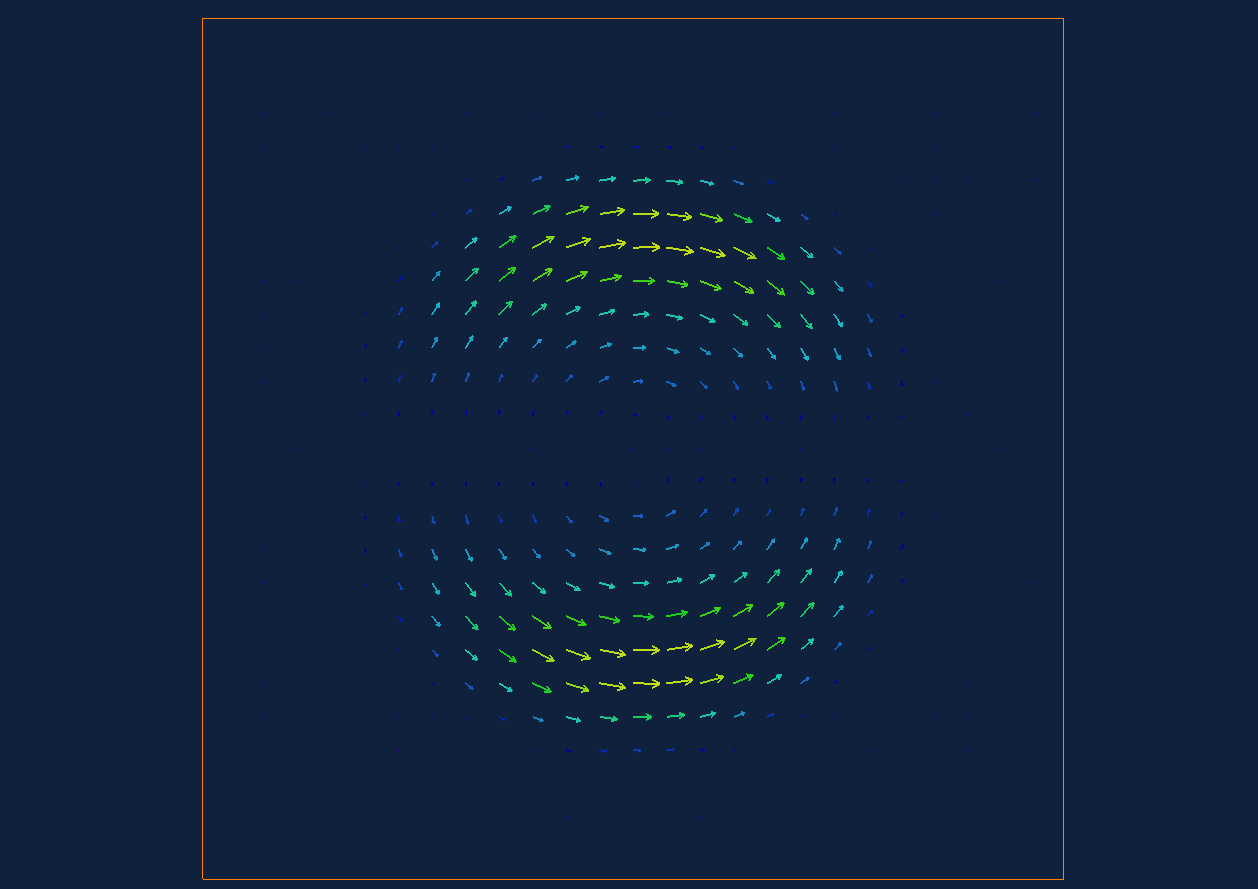
\includegraphics[width=.48\textwidth,clip,trim=5.5cm 1cm 5.5cm 1cm]{./Rezultati/p1_mode1}}
 \subfigure{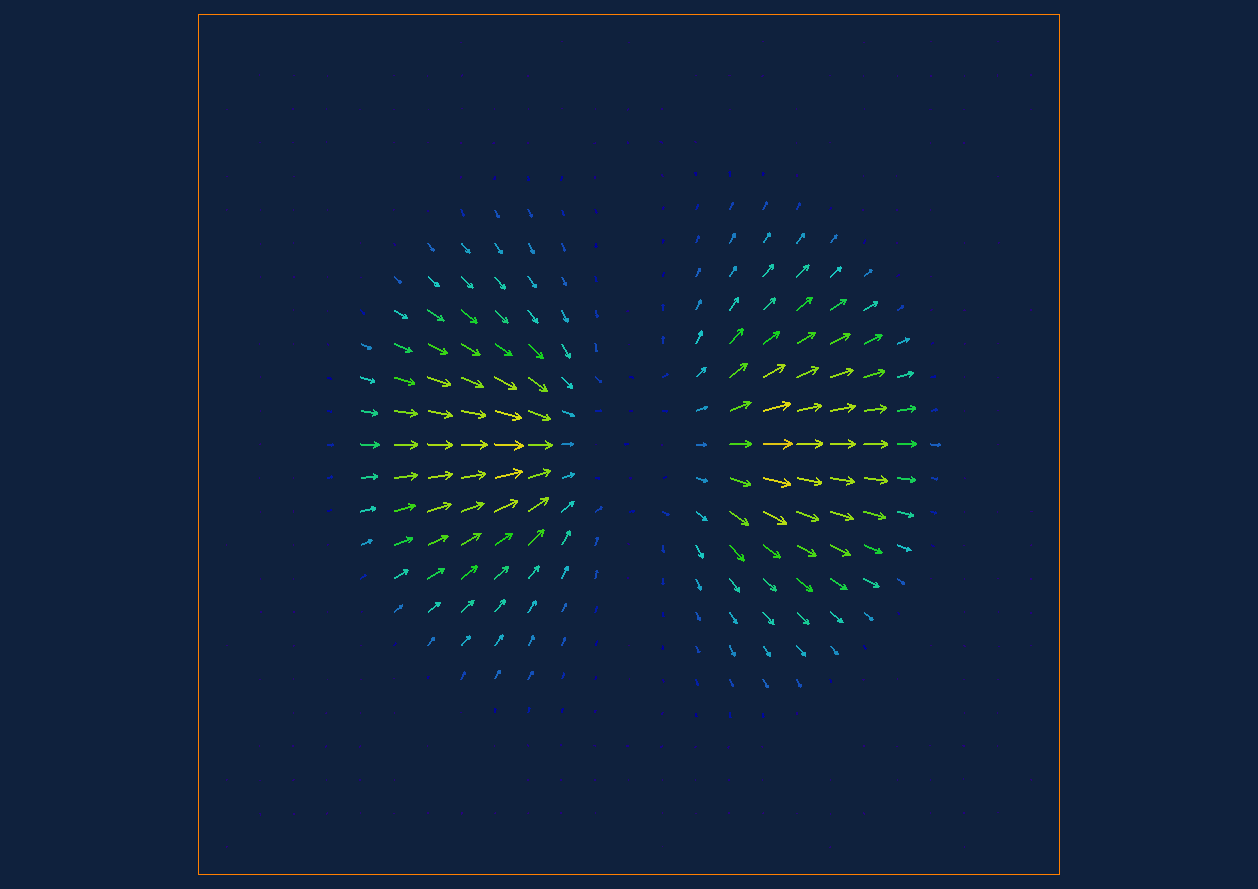
\includegraphics[width=.48\textwidth,clip,trim=5.5cm 1cm 5.5cm 1cm]{./Rezultati/p1_mode2}}
 \caption{Lastna na"cina "sirjenja svetlobe skozi vlakno z radialnim profilom direktorja ($s=+1$)}
 \label{fig:pulse-p1-mode}
\end{figure}

S slike takoj opazimo podobnost med polarizacijo svetlobe, zlasti pri po"casnej"sem nihajnem na"cinu (slika \ref{fig:pulse-p1-mode} desno), in direktorskim poljem. 
"Ce na polarizacijo gledamo kot na vektor brez pu"s"cice, lahko z ena"cbo (\ref{eq:winding-number}) obema na"cinoma priredimo ovojno "stevilo $+1$. 
Dodatno pa imata oba na"cina "se zrcalno ravnino, kjer se polarizacija svetlobe obrne. 
V enem izmed na"cinov je ta ravnina navpi"cna, v drugem pa vodoravna. 
"Ce polarizacijo svetlobe na eni strani te ravnine obrnemo, dobimo pravi linijski defekt mo"ci $+1$. 

Direktosko polje znotraj vlakna ima radialno simetrijo, saj se ne spremeni "ce vlakno vrtimo okrog svoje osi. 
To simetrijo pa zlomi vpadna svetloba, ki uvede preferen"cno smer, in sicer smer polarizacije. 
Po dolgem "casu v vlaknu mora svetlobni "zarek zadostiti obem simetrijam. 
Oba na"cina na sliki \ref{fig:pulse-p1-mode} si lahko predstavljamo kot defekta z ovojnim "stevilom $+1$, ki jim odstranimo vse tiste dele, kjer bi polarizacija morala kazati pravokotno na vpadno polarizacijo. 

\subsection{Hiperboli"cni profil direktorja}

V vlaknu z radialnim direktorskim profilom opazimo tesno povezavo med simetrijo teko"cega kristala in polarizacijo svetlobe. 
Na podlagi tega lahko pri"cakujemo podobno povezavo tudi, "ce namesto defekta z ovojnim "stevilom $+1$ v sredino vlakna postavimo drug defekt. 
Z vektorskim poljem so kompatibilni le tak"sni s celo"stevilsko mo"cjo, zato sem izbraj hiperboli"cni defekt z $s=-1$. 

Kratek laserski sunek se podobno kot pri radialnem profilu razdeli na dva na"cina, ki sta skladna s simetrijo direktorja. 
Oba na"cina sta prikazana na sliki \ref{fig:pulse-m1-mode}. 

\begin{figure}[h]
 \centering
 \subfigure{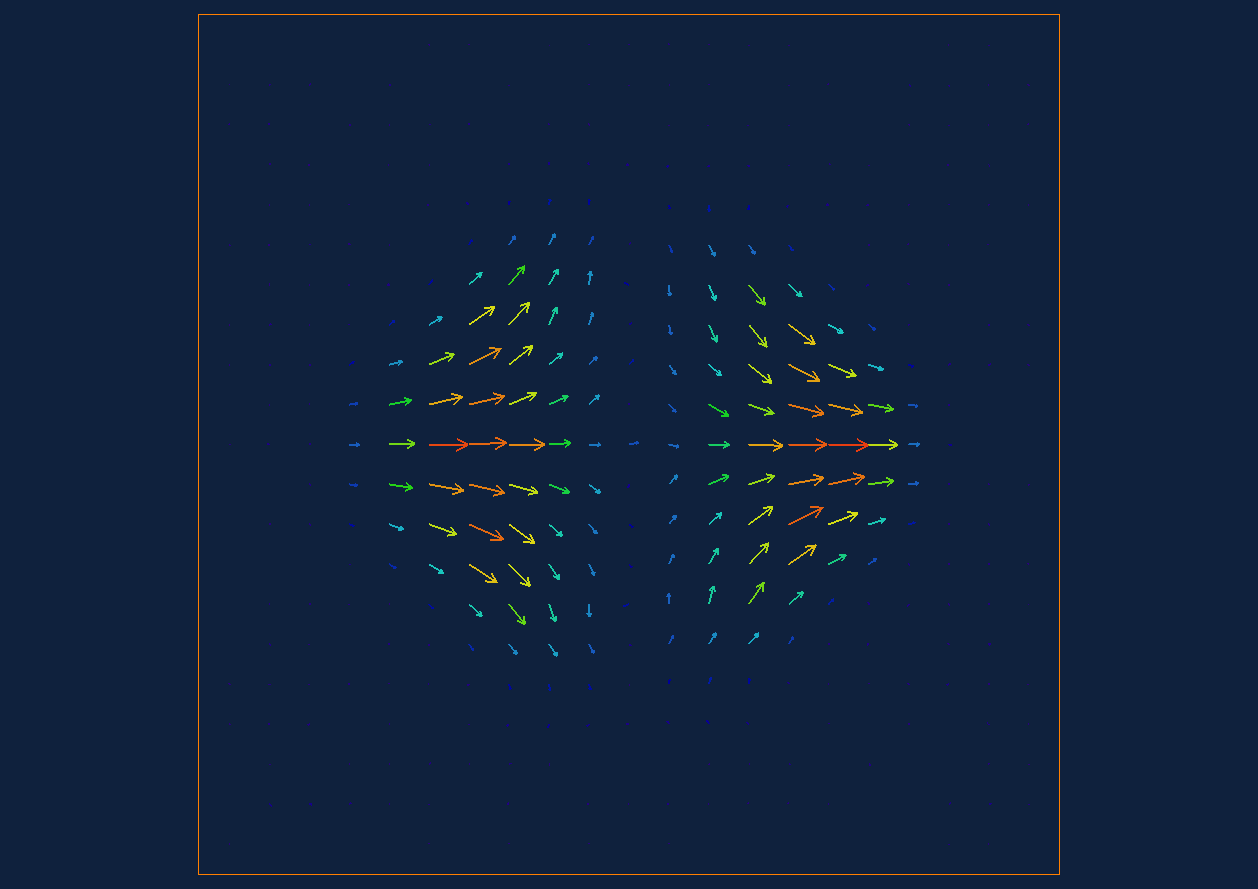
\includegraphics[width=.48\textwidth,clip,trim=5.5cm 1cm 5.5cm 1cm]{./Rezultati/m1_mode1}}
 \subfigure{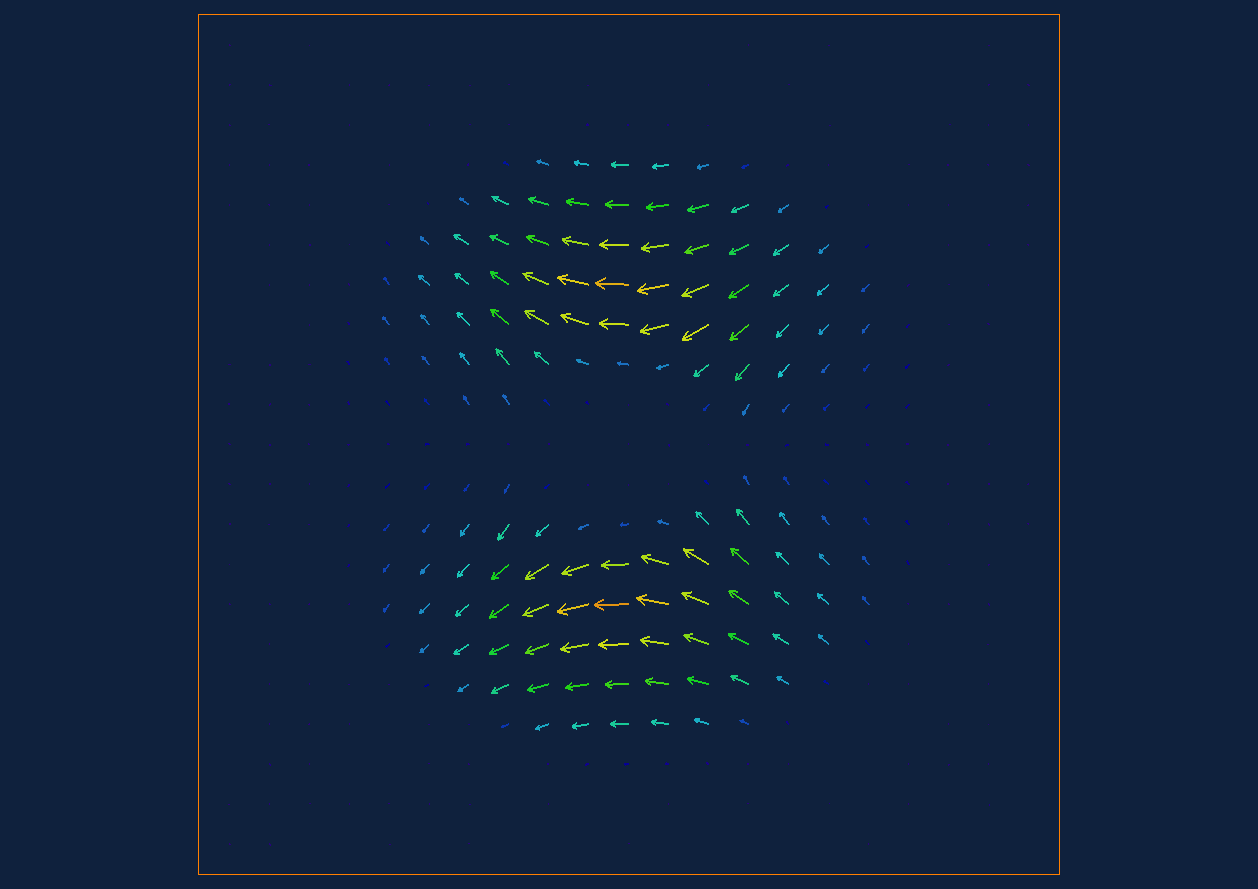
\includegraphics[width=.48\textwidth,clip,trim=5.5cm 1cm 5.5cm 1cm]{./Rezultati/m1_mode2}}
 \caption{Lastna na"cina "sirjenja svetlobe skozi vlakno s hiperboli"cnim profilom direktorja ($s=-1$)}
 \label{fig:pulse-m1-mode}
\end{figure}

Obmo"cja z vi"sjo intenziteto svetlobe so razporejena enako kot na sliki \ref{fig:pulse-p1-mode}, polarizacijo svetlobe pa tvori defekt z ovojnim "stevilom $-1$. 
Spet sta vidni ravnini brez svetlobe, kjer se smer polarizacije obrne. 

\subsection{Defekti z necelo mo"cjo}

Videli smo, da radialni in hiperboli"cni profil direktorja znotraj teko"cekristalnega vlakna vsili svojo simetrijo svetlobi. 
Na mestih, kjer ta simetrija ni kompatibilna s polarizacijo vpadne svetlobe, svetlobe ni. 
V obeh primerih bi lahko z obratom polarizacije na delu vlakna dosegli, da polarizacija svetlobe tvori defekt s celo"stevilsko mo"cjo. 
Tak"sni defekti so kompatibilni z vektorskimi polji, kot je elektri"cno polje svetlobe. 

V teko"cem kristalu pa lahko ustvarimo tudi defekte s polcelo mo"cjo, ki jih prava vektorska polja ne morejo tvoriti. 
Simuliral sem "sirjenje svetlobe skozi teko"cekristalno vlakno, ki ima v osi linijski defekt z ovojnim "stevilom $s \pm 1/2$. 

Izkazalo se je, da se tudi v tem primeru laserski sunek razcepi na dva dela, ki ustrezata redni in izredni polarizaciji. 

\begin{figure}[h]
 \centering
 \subfigure{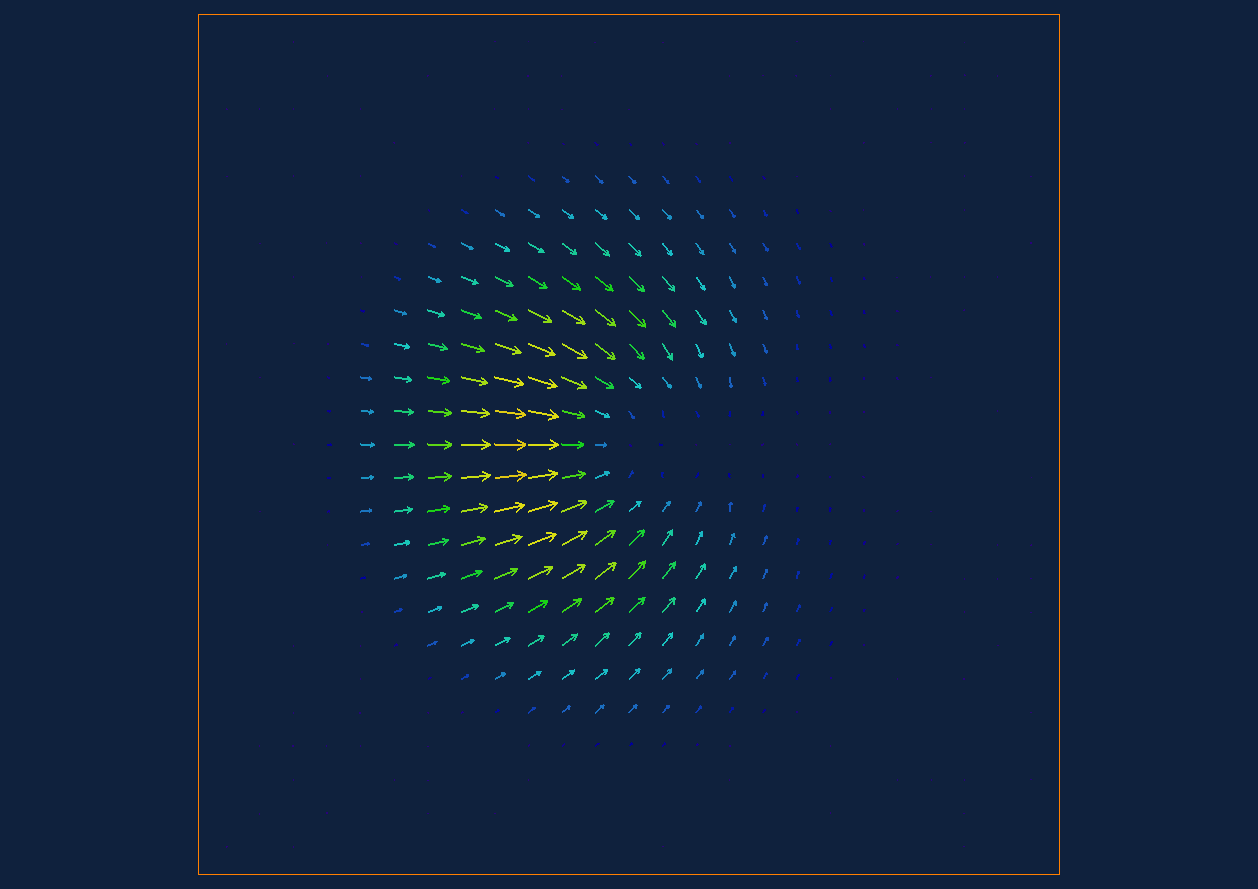
\includegraphics[width=.48\textwidth,clip,trim=5.5cm 1cm 5.5cm 1cm]{./Rezultati/p12_mode1}}
 \subfigure{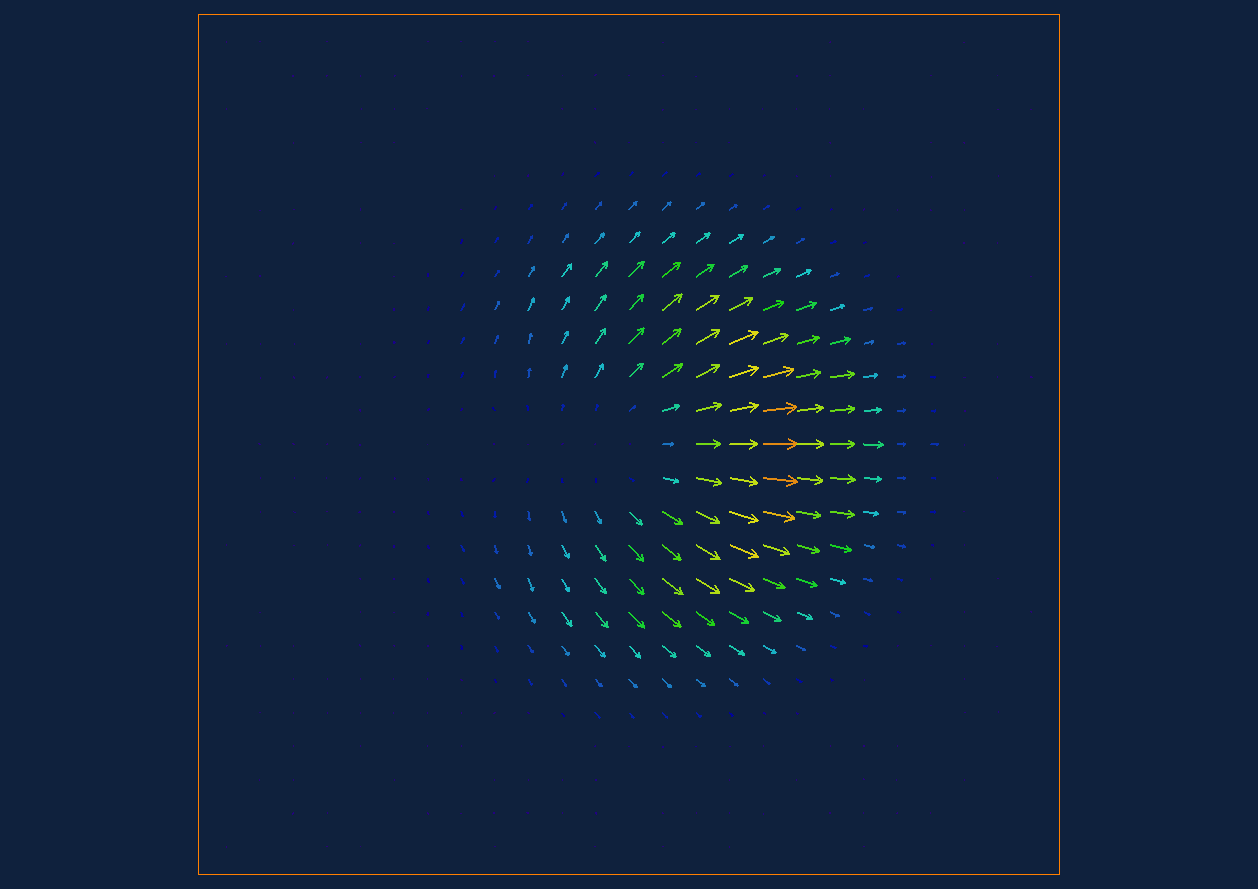
\includegraphics[width=.48\textwidth,clip,trim=5.5cm 1cm 5.5cm 1cm]{./Rezultati/p12_mode2}}
 \caption{Lastna na"cina "sirjenja svetlobe skozi vlakno z defektom z necelim ovojnim "stevilom $s=+1/2$}
 \label{fig:pulse-p12-mode}
\end{figure}

\begin{figure}[h]
 \centering
 \subfigure{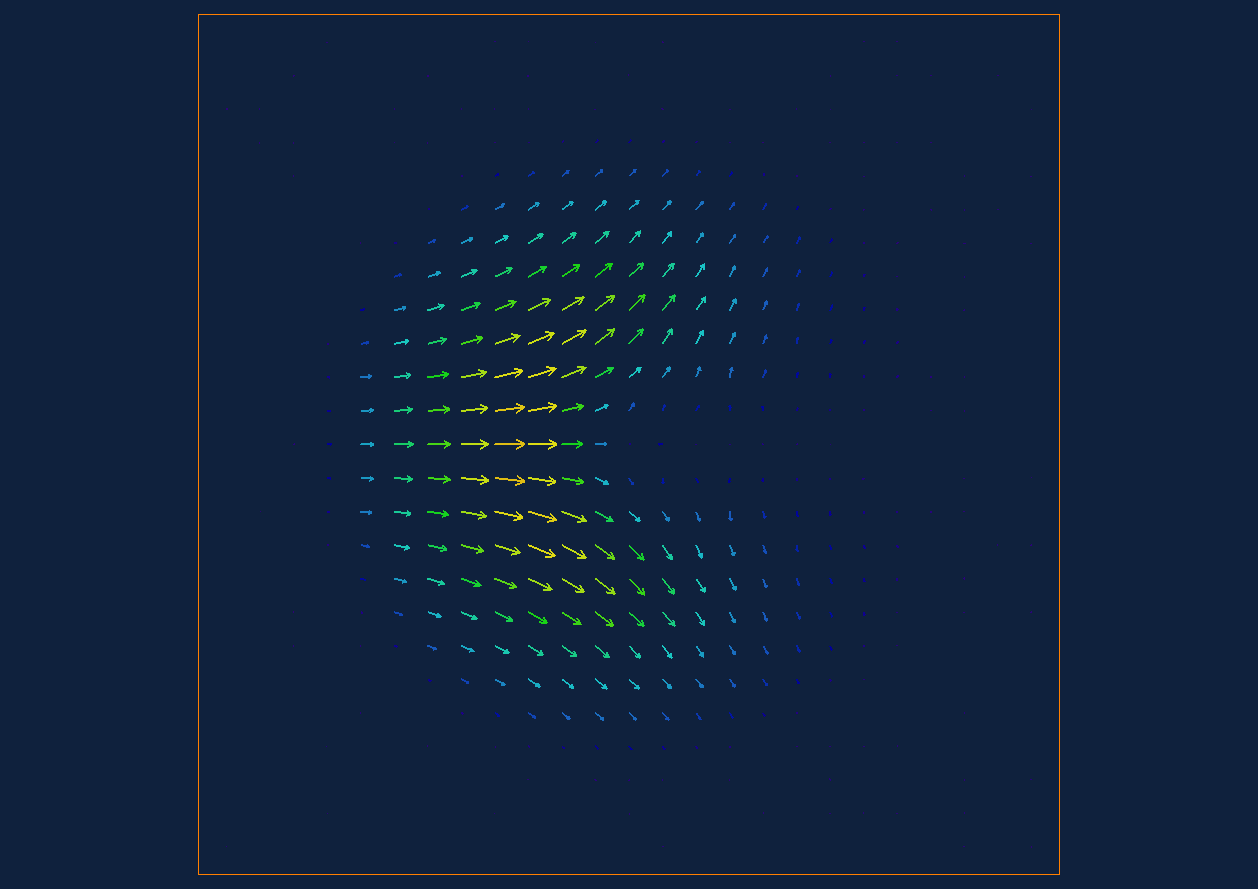
\includegraphics[width=.48\textwidth,clip,trim=5.5cm 1cm 5.5cm 1cm]{./Rezultati/m12_mode1}}
 \subfigure{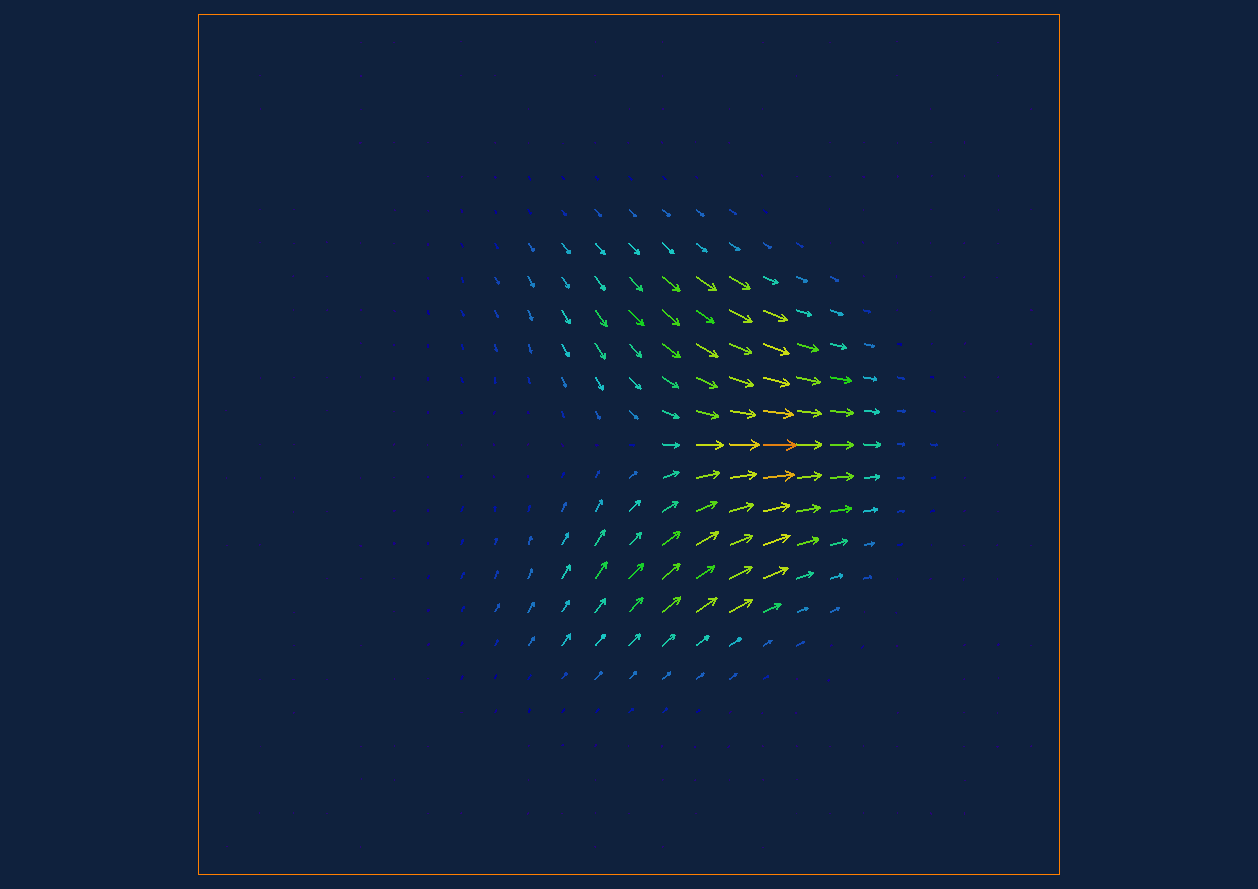
\includegraphics[width=.48\textwidth,clip,trim=5.5cm 1cm 5.5cm 1cm]{./Rezultati/m12_mode2}}
 \caption{Lastna na"cina "sirjenja svetlobe skozi vlakno z defektom z necelim ovojnim "stevilom $s=-1/2$}
 \label{fig:pulse-m12-mode}
\end{figure}

V nasprotju z radialnim in hiperboli"cnim profilom pri propagaciji svetlobe skozi defekte z necelo mo"cjo ne opazimo ravnin brez svetlobe. 
Znotraj vsakega lastnega na"cina je le eno intenzitetno obmo"cje. 

\subsection{Splo"sne zakonitosti}
Na podlagi vseh zgorjih opa"zanj lahko najdemo podobnosti in izpeljemo splo"sne zakonitosti. 

\begin{itemize}
 \item Pulz linearno polarizirane svetlobe se vedno razdeli na dva lastna na"cina, ki ustrezata redni in izredni polarizaciji.
 \item Polarizacija svetlobe v obeh na"cinih tvori defekt z enakim ovojnim "stevilom kot defekt v teko"cem kristalu.
 \item V enem izmed na"cinov je polarizacija svetlobe vzporedna z direktorjem, v drugem pa je nanj pravokotna.
 \item V obmo"cjih, kjer bi po prej"snjem pravilu morala biti svetloba polarizirana pravokotna na vpadno polarizacijo, svetlobe ni. 
\end{itemize}

S pomo"cjo teh zakonitosti lahko napovemo, kako se bo svetloba "sirila po vlaknu s poljubni linijskim defektom po sredini. 


\section{Zaklju"cek}

\newpage
\bibliographystyle{zumer}
\bibliography{magisterij}

\end{document}
